% %%%%%%%%%%%%%%%%%%%%%%%%%%%
% % Systematic uncertainties
% %%%%%%%%%%%%%%%%%%%%%%%%%%%

 
The input to the statistical analysis is an ensemble of histograms in the $(\mr,\rsq)$ plane that 
incorporates systematic uncertainties in the simulated signal and background samples.  
The independent systematic effects, described below, are sampled simultaneously. 
This is one of the characteristics that sets this analysis apart. 
For each sampled systematic effect, the same zero mean, unit variance, Gaussian variate is used in
the calculation of the random shift of the systematic effect for all the signal and background
models. Likewise, the same randomly sampled parton distribution functions are used for all
signal and background models. 
In this way, the statistical dependencies among all bins of the signal and background models are
correctly, and automatically, modelled. The sampling of the systematic effects
is repeated several hundred ($N$) times.  
In all cases, except for the PDFs, the systematic uncertainties are in the scale factors (SF) 
applied to the simulated samples to correct them for modelling deficiencies. 
In the next subsections I will discuss each source of systematic uncertainty in more detail. 

%\vspace{1eM}

% TODO merge/divide with object id section
%\textcolor{red}{Some of this information might be moved to the event reconstruction and object
%ID section.}

%\vspace{1eM}

%%%%%%%%%%%%%%%%%%%%%%%%%%%%%%%%%%%%%%%%%%%%%%%%%%%%%%%%%%%%%%%%%%%%%%%%%%%%%%%%%%%%%%%%%%%%%%%%%%%%
\subsection{Jet energy scale corrections \label{sec:boost_JEC}}  

Jet energy scale corrections (JEC) map the measured jet energy deposition in the detector back to
the particle level. Within CMS the JEC are applied in sequential levels, each correcting for a
different effect. Details on the various levels were given in Section~\ref{sec:object_jets}.
For our discussion here, the important thing to remember is that each level of correction is simply
a scaling of the four-momentum of the jet by a scale factor that depends on the jet \pt and $\eta$.

Uncertainties on JEC originate from various uncorrelated sources.   
Given $M$ such sources, the full correction on the \pt of a jet, according to a random shift
within the uncertainties, becomes 
\begin{equation}
s(\pt, \eta, \alpha_i) = \sum_{i=1}^M \alpha_i S_i (\pt, \eta)
\end{equation}
where $S_i (\pt, \eta)$ is a \pt and $\eta$-dependent JEC uncertainty for a source $i$ and
$\alpha_i$ are weights randomly sampled from a Gaussian distribution with zero mean and unit
width. 
Here, the weights $\alpha_i$ are different for each source, but are universal for each jet and each
event when considering a given systematic sampling.
Dealing with the myriad of uncertainty sources is not so straight-forward in practice, and also not
necessary for a new physics search. As recommended by the POG providing the jet energy scale
corrections and uncertainties, we will therefore take on a much simpler approach, using a total
uncertainty $S (\pt, \eta)$ and a random number $\alpha$ from a single Gaussian,
\begin{equation}
s(\pt, \eta, \alpha) = \alpha S (\pt, \eta) = \alpha \sqrt {\sum_i^M s_i^2 (\pt, \eta) }.
\end{equation}
The jet $p_T$ for a given random variation becomes:
\begin{equation}
\pt^{\rm corr} = \left(1 + s(\pt, \eta, \alpha)\right) \pt^{\rm orig}.
\end{equation}
This calculation is repeated $N$ times, each time, using a different number sampled from the
Gaussian.  
The overall effect of the JEC uncertainty on the yield is obtained from the distribution of
resulting $N$ yields.  
As for the jet energy scale corrections themselves, the associated uncertainties are also
propagated to the \VEtmiss.


%%%%%%%%%%%%%%%%%%%%%%%%%%%%%%%%%%%%%%%%%%%%%%%%%%%%%%%%%%%%%%%%%%%%%%%%%%%%%%%%%%%%%%%%%%%%%%%%%%%%
\subsection{Parton distribution functions \label{sec:boost_pdf_unc}} 

In order to evaluate the systematic uncertainty arising from imperfect knowledge of the parton
distribution functions, we use three PDF sets, {\tt MSTW2008lo68cl}~\cite{Martin:2009iq},
{\tt CT10}~\cite{Lai:2010vv}, and {\tt NNPDF23\_lo\_as\_0130\_qed}~\cite{nnpdf}, which are
recommended by the PDF4LHC group~\cite{Alekhin:2011sk,Botje:2011sn}.  
Since we take into account full correlations within systematic variations, we need a way to sample
randomly also from the PDF uncertainties, such that the PDF variations can be incorporated directly
in our workflow. 
Of the three recommended PDF sets, {\tt NNPDF} presents the PDF eigenvectors as a randomly
distributed set, while the other groups provide eigenvectors obtained by varying the PDF fit
parameters by $\pm 1$ standard deviation.  
However, the recently developed {\tt LHAPDF6}~\cite{LHAPDF6} offers a formal way to convert the
latter sets into the randomly distributed sets we need.  
We have used the program {\tt hessian2replicas} to generate randomly
distributed PDF sets with 100 members each, for both {\tt CT10} and {\tt MSTW2008lo68cl}.  

Given a sampled set $i$, for PDF set $K$, and the PDF set $O$ with which the events were simulated,
events are reweighted using the scale factors, 
\begin{equation}
{\rm SF}_{K, i} = \frac{w_{K, i}}{w_{O}},
\end{equation}
where the weights $w$ are products of the event-by-event PDFs for both colliding partons.
The PDF set $O$ was listed for each sample in Section~\ref{sec:boost_mc_samples}.
The overall PDF uncertainty on the background counts or signal efficiencies is derived
from the distribution of ${\rm SF}_{K, i}$ obtained by a random selection of $K$ and $i$.  

To study the effect of the different PDF sets on the simulated counts used in the background
estimation, we compute the distribution of simulated counts corresponding to a random selection of
PDF members from the three considered PDF sets. 
A Gaussian distribution is then fitted to these distributions. Its width indicates the uncertainty
induced by the given PDF set. 
Figures~\ref{fig:PDF_effect_on_bg_QCD}-\ref{fig:PDF_effect_on_bg_oth2} show the result of this
procedure for the simulated background counts that are used to compute the translation factors
$\kappa$. 
There is a Gaussian distribution for each PDF set, and the arrow indicates the value for a given
count as obtained using the PDF set that was used during the generation of the MC samples. 
From these figures we conclude that the overall systematic uncertainty resulting from the parton
distribution functions on the background counts is due to both the difference in the nominal values
of the PDF sets, and the spread within the separate PDF sets.

Figure~\ref{fig:PDF_effect_on_sig} shows the equivalent for an example signal point. Here we see
that the spread of the {\tt CT10} PDF dominates the total uncertainty on the signal efficiency. 
We also note that we have computed the signal efficiencies with respect to the nominal PDF set
member of the considered PDF rather than the original PDF used for the generation of the samples.
This is done to make sure that only the PDF effects on the acceptance are included in the
experimental uncertainties. The PDF effect on the expected signal cross section is taken into
account separately.

\begin{figure}[htpb]
\centering
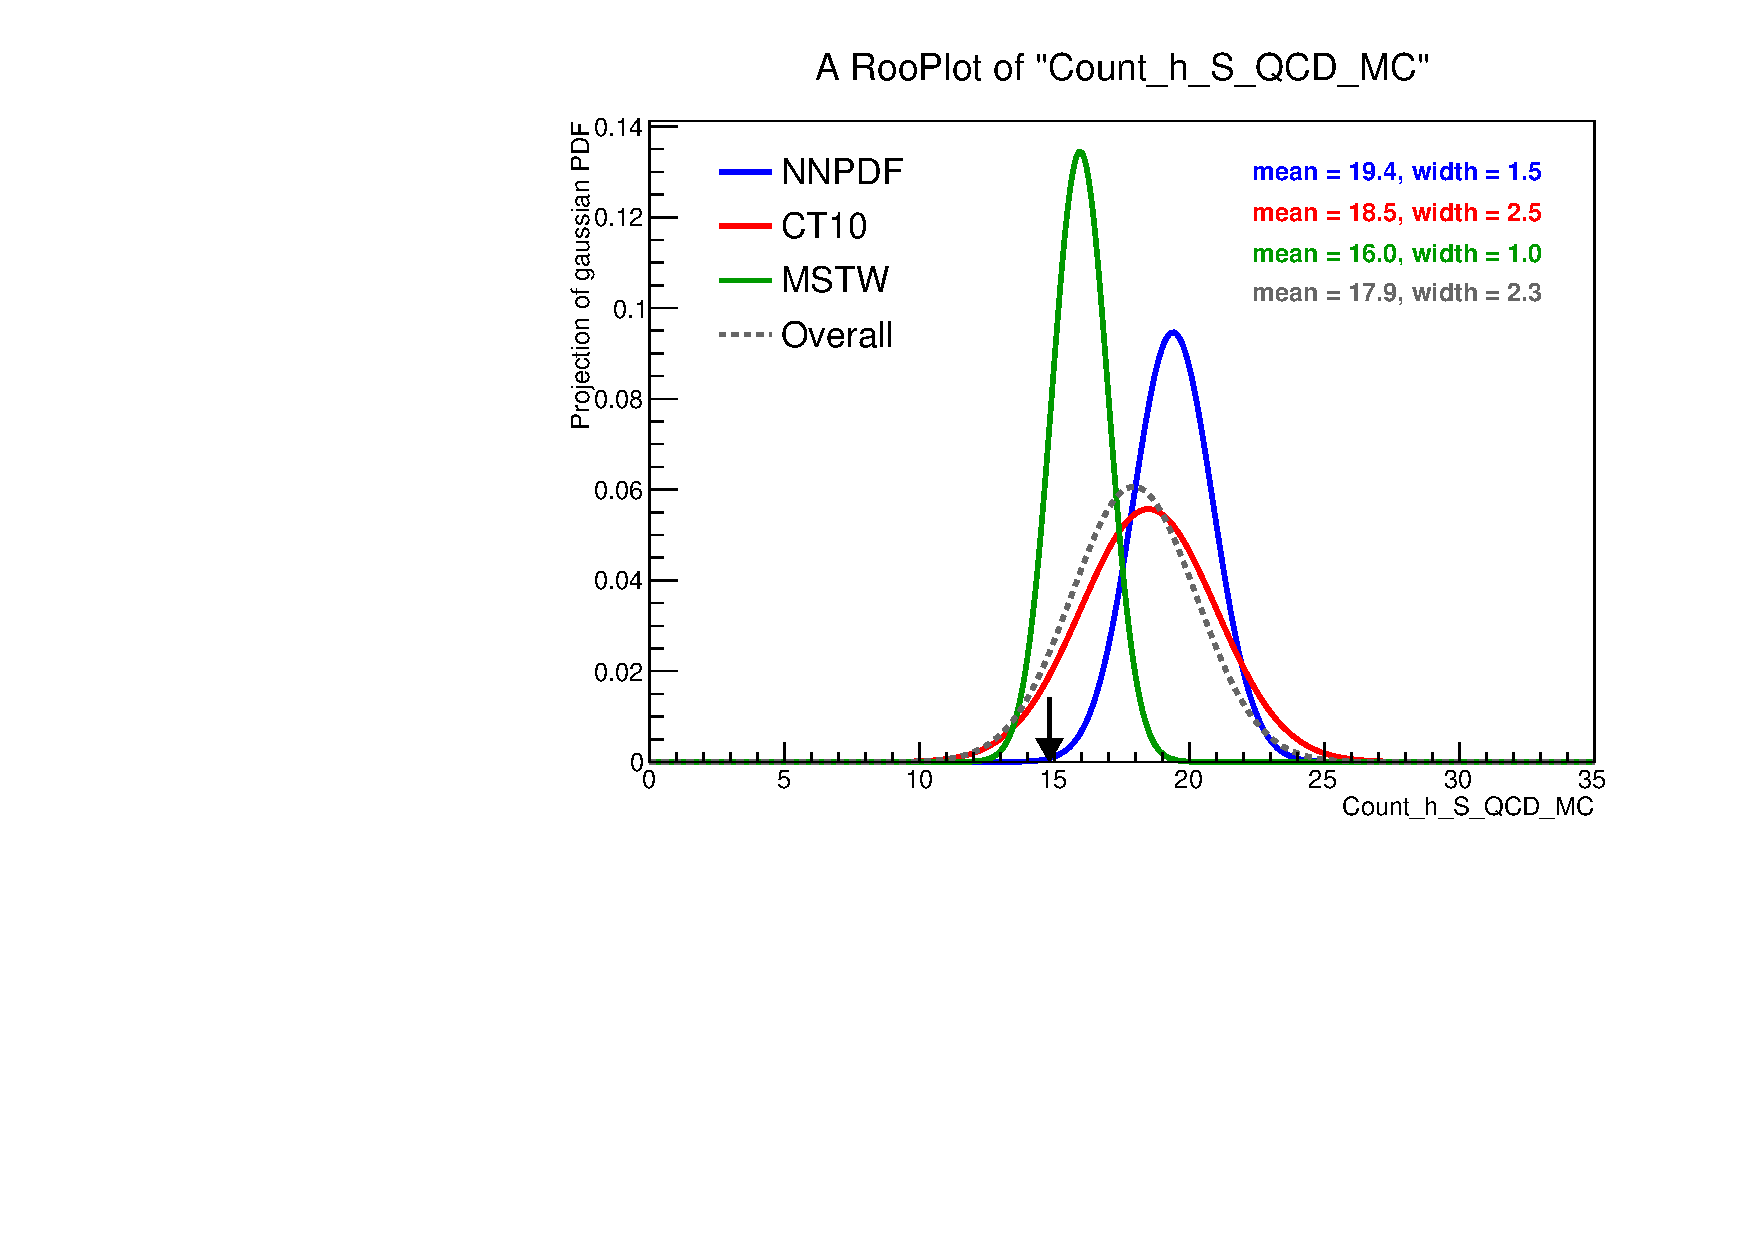
\includegraphics[width=0.48\textwidth,clip=true,trim=0 0.2cm 0 1.2cm]
{figures/razor_systematics/h_S_QCD_MC}
~
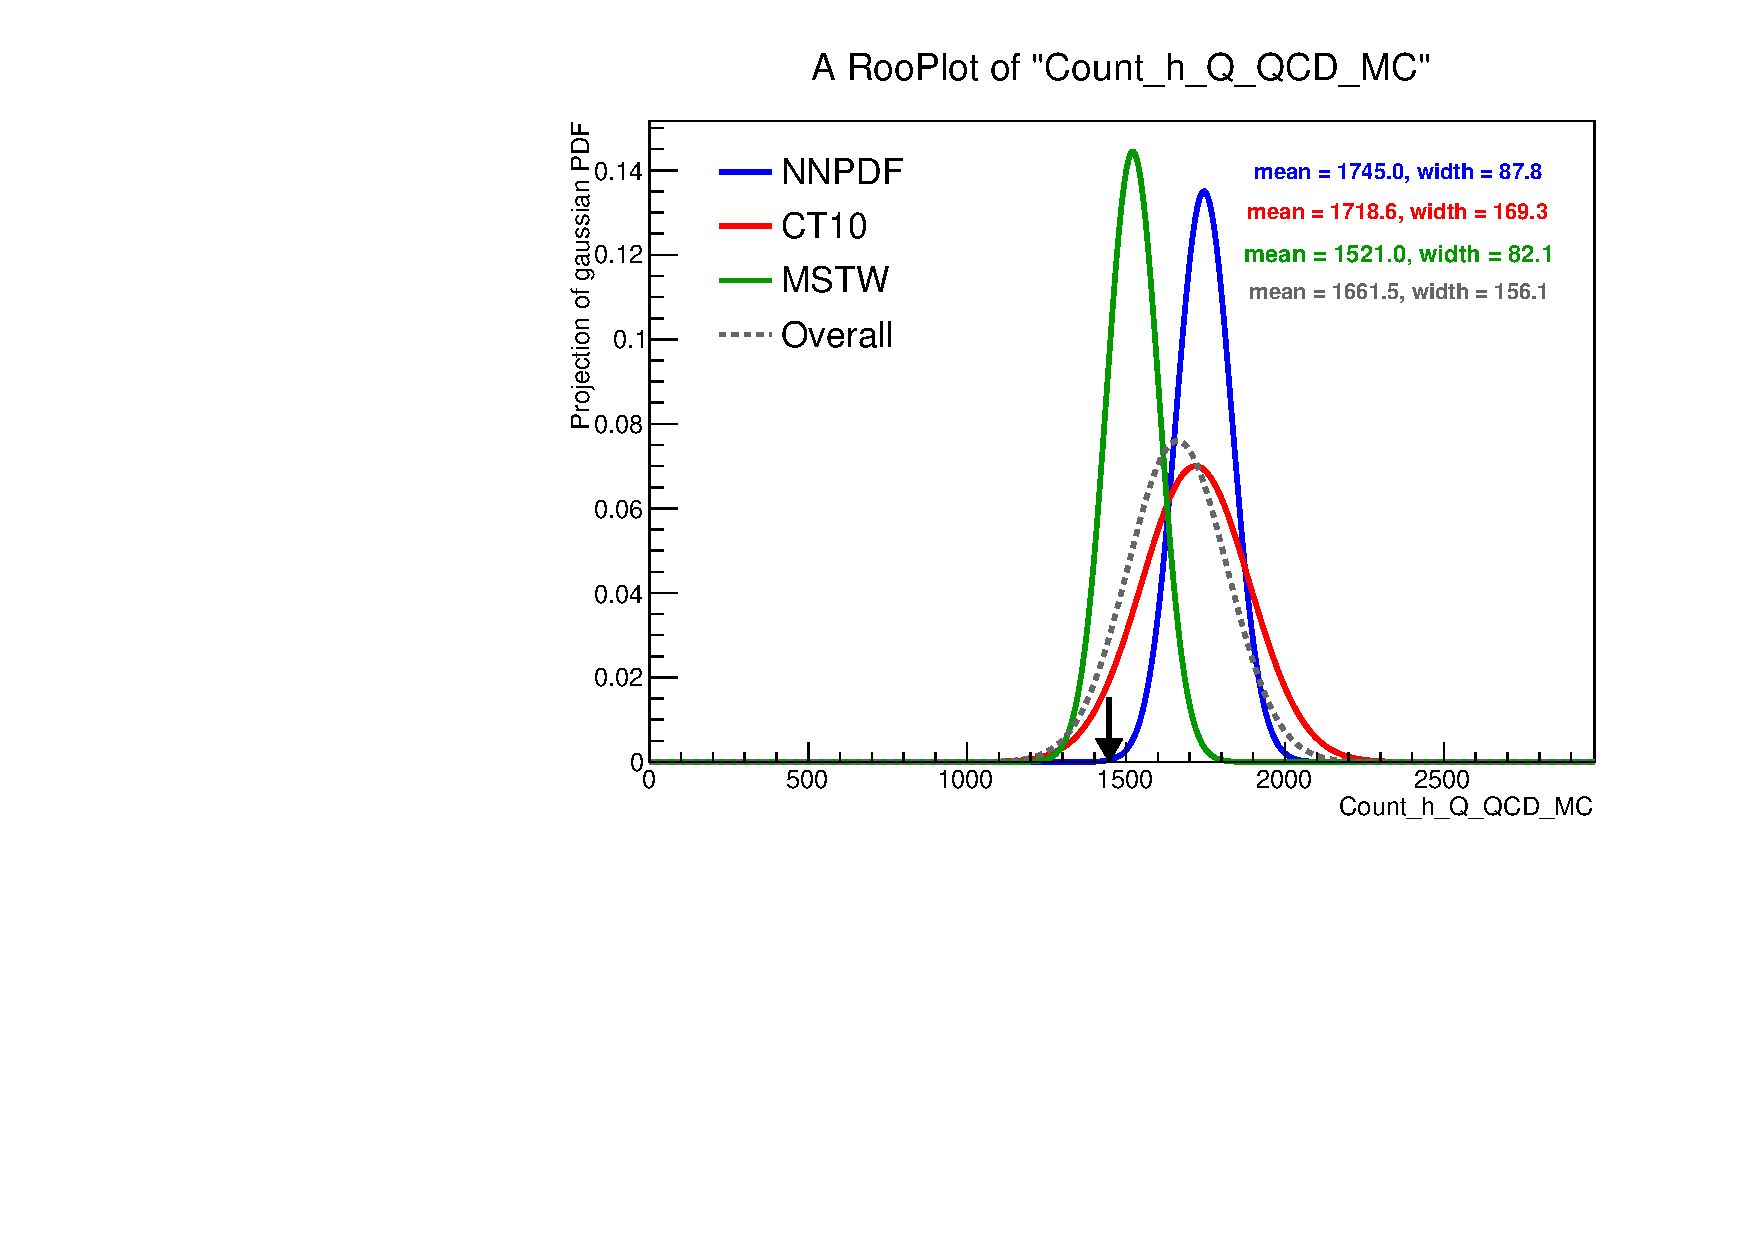
\includegraphics[width=0.48\textwidth,clip=true,trim=0 0.2cm 0 1.2cm]
{figures/razor_systematics/h_Q_QCD_MC}
\caption{Influence of different PDF sets on the MC counts entering $\kappa_{QCD}^{Q/S}$
\label{fig:PDF_effect_on_bg_QCD}}
\end{figure}

\begin{figure}[htpb]
\centering
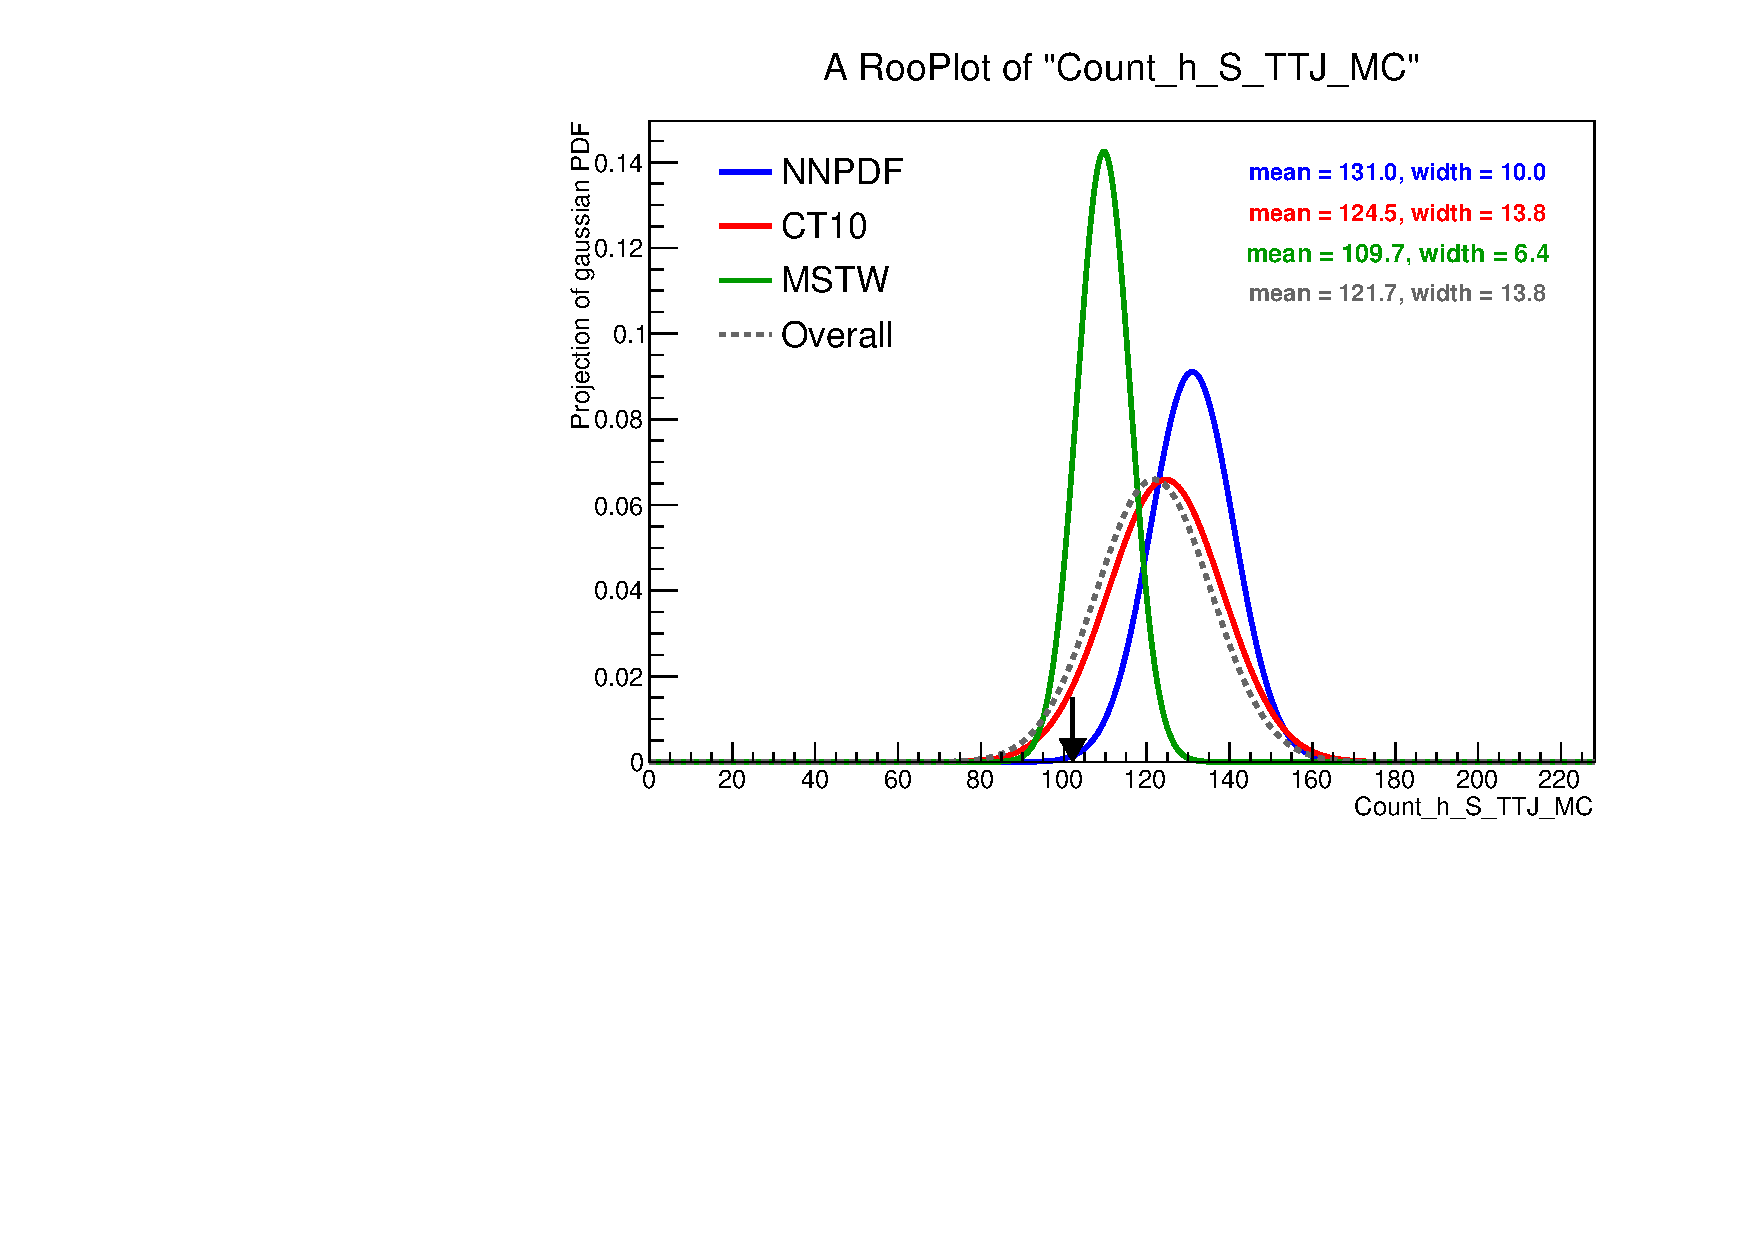
\includegraphics[width=0.48\textwidth,clip=true,trim=0 0.2cm 0 1.2cm]
{figures/razor_systematics/h_S_TTJ_MC}
~
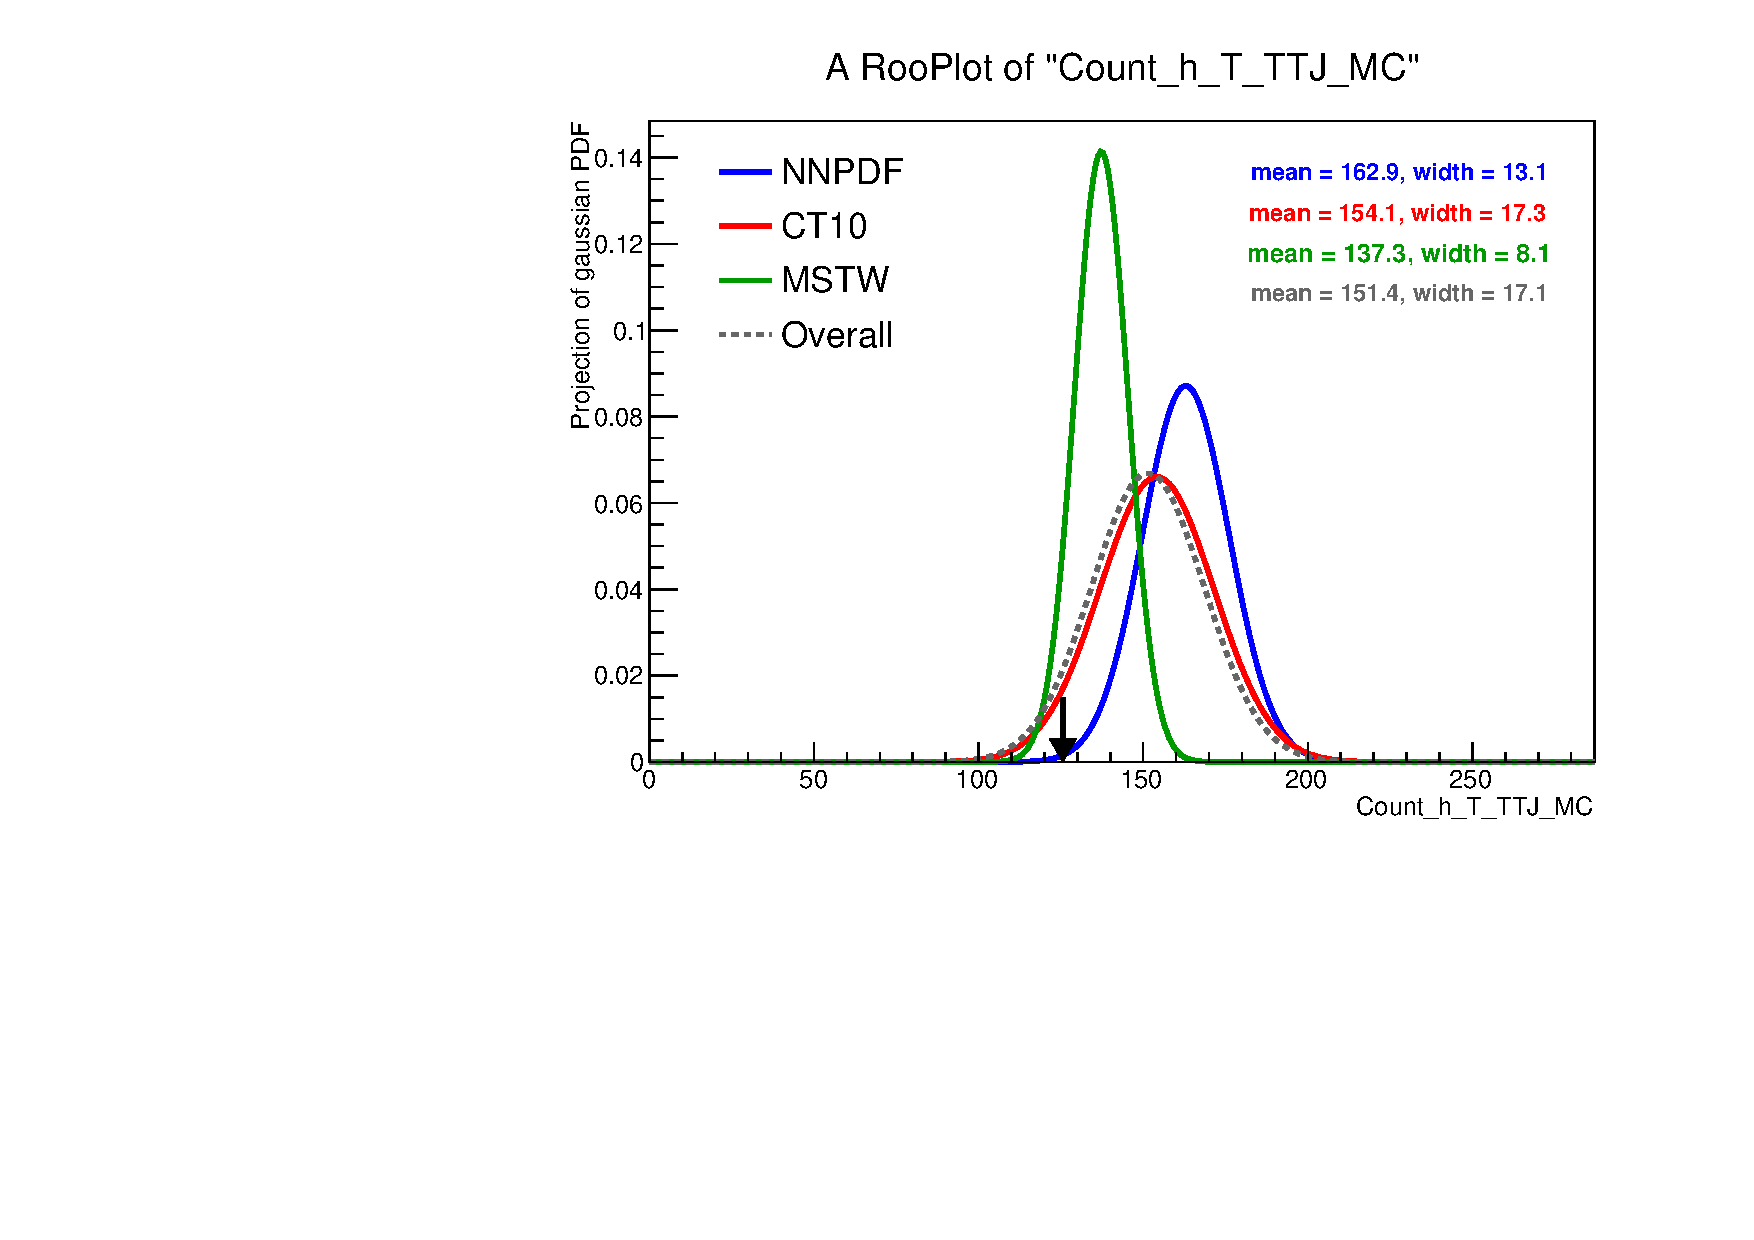
\includegraphics[width=0.48\textwidth,clip=true,trim=0 0.2cm 0 1.2cm]
{figures/razor_systematics/h_T_TTJ_MC}
\caption{Influence of different PDF sets on the MC counts entering $\kappa_{TTJ}^{T/S}$
\label{fig:PDF_effect_on_bg_TTJ}}
\end{figure}

\begin{figure}[htpb]
\centering
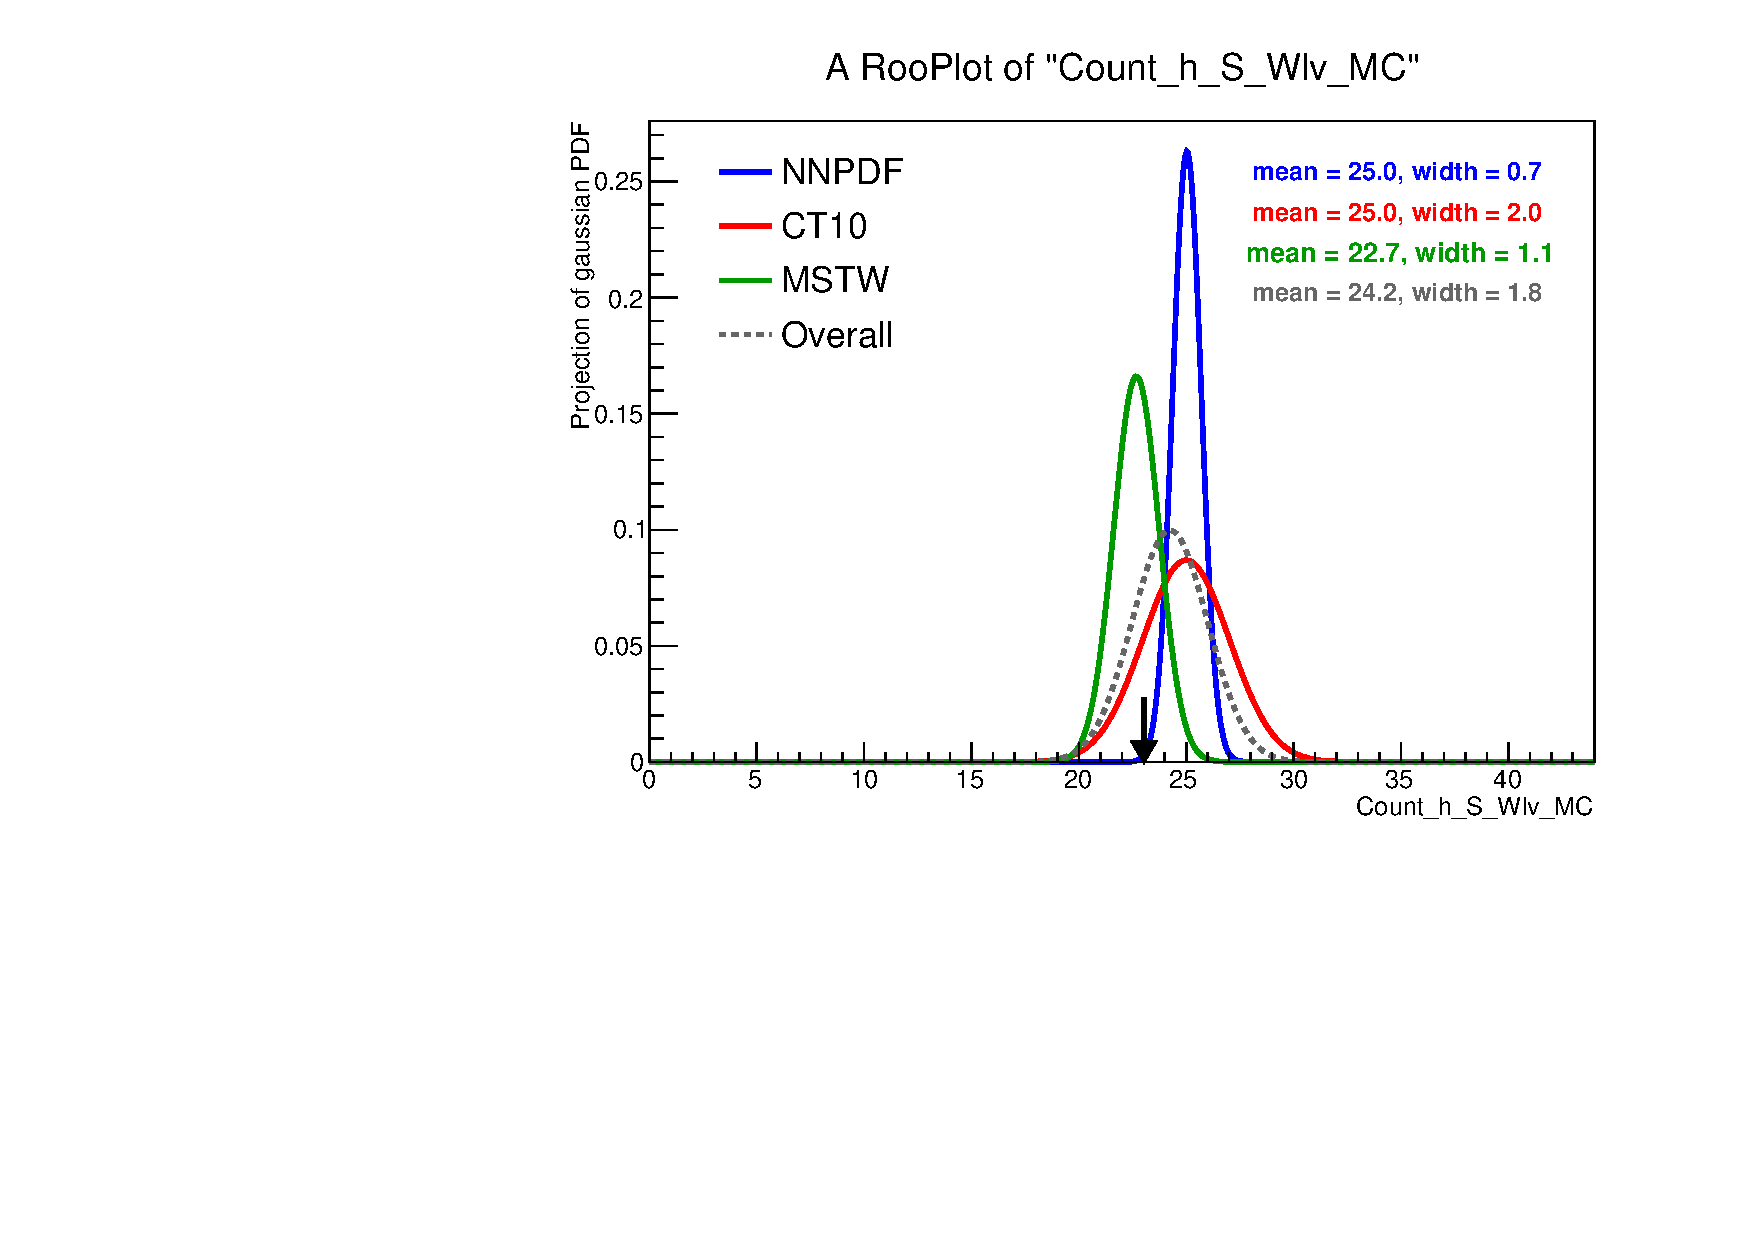
\includegraphics[width=0.48\textwidth,clip=true,trim=0 0.2cm 0 1.2cm]
{figures/razor_systematics/h_S_Wlv_MC}
~
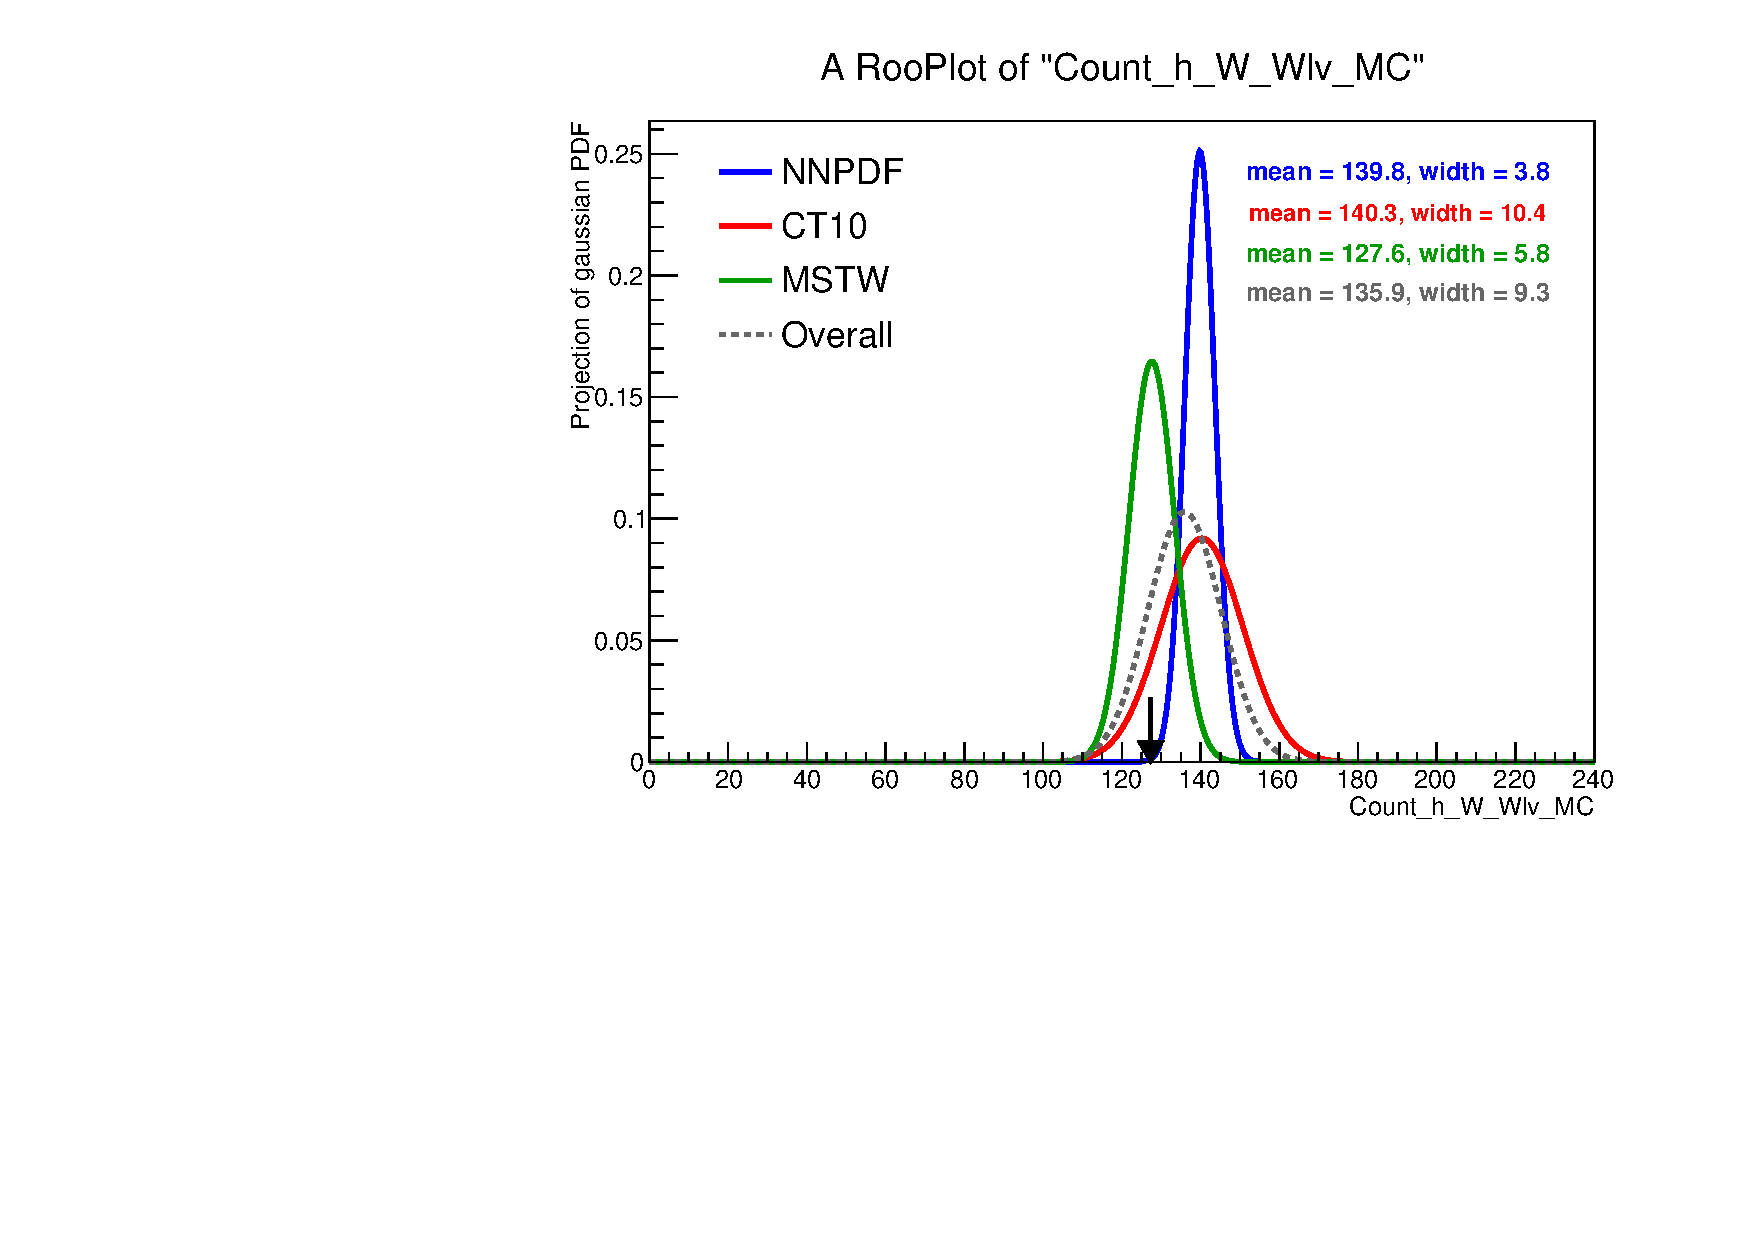
\includegraphics[width=0.48\textwidth,clip=true,trim=0 0.2cm 0 1.2cm]
{figures/razor_systematics/h_W_Wlv_MC}
\caption{Influence of different PDF sets on the MC counts entering $\kappa_{Wlv}^{W/S}$
\label{fig:PDF_effect_on_bg_Wlv}}
\end{figure}


\begin{figure}[htpb]
\centering
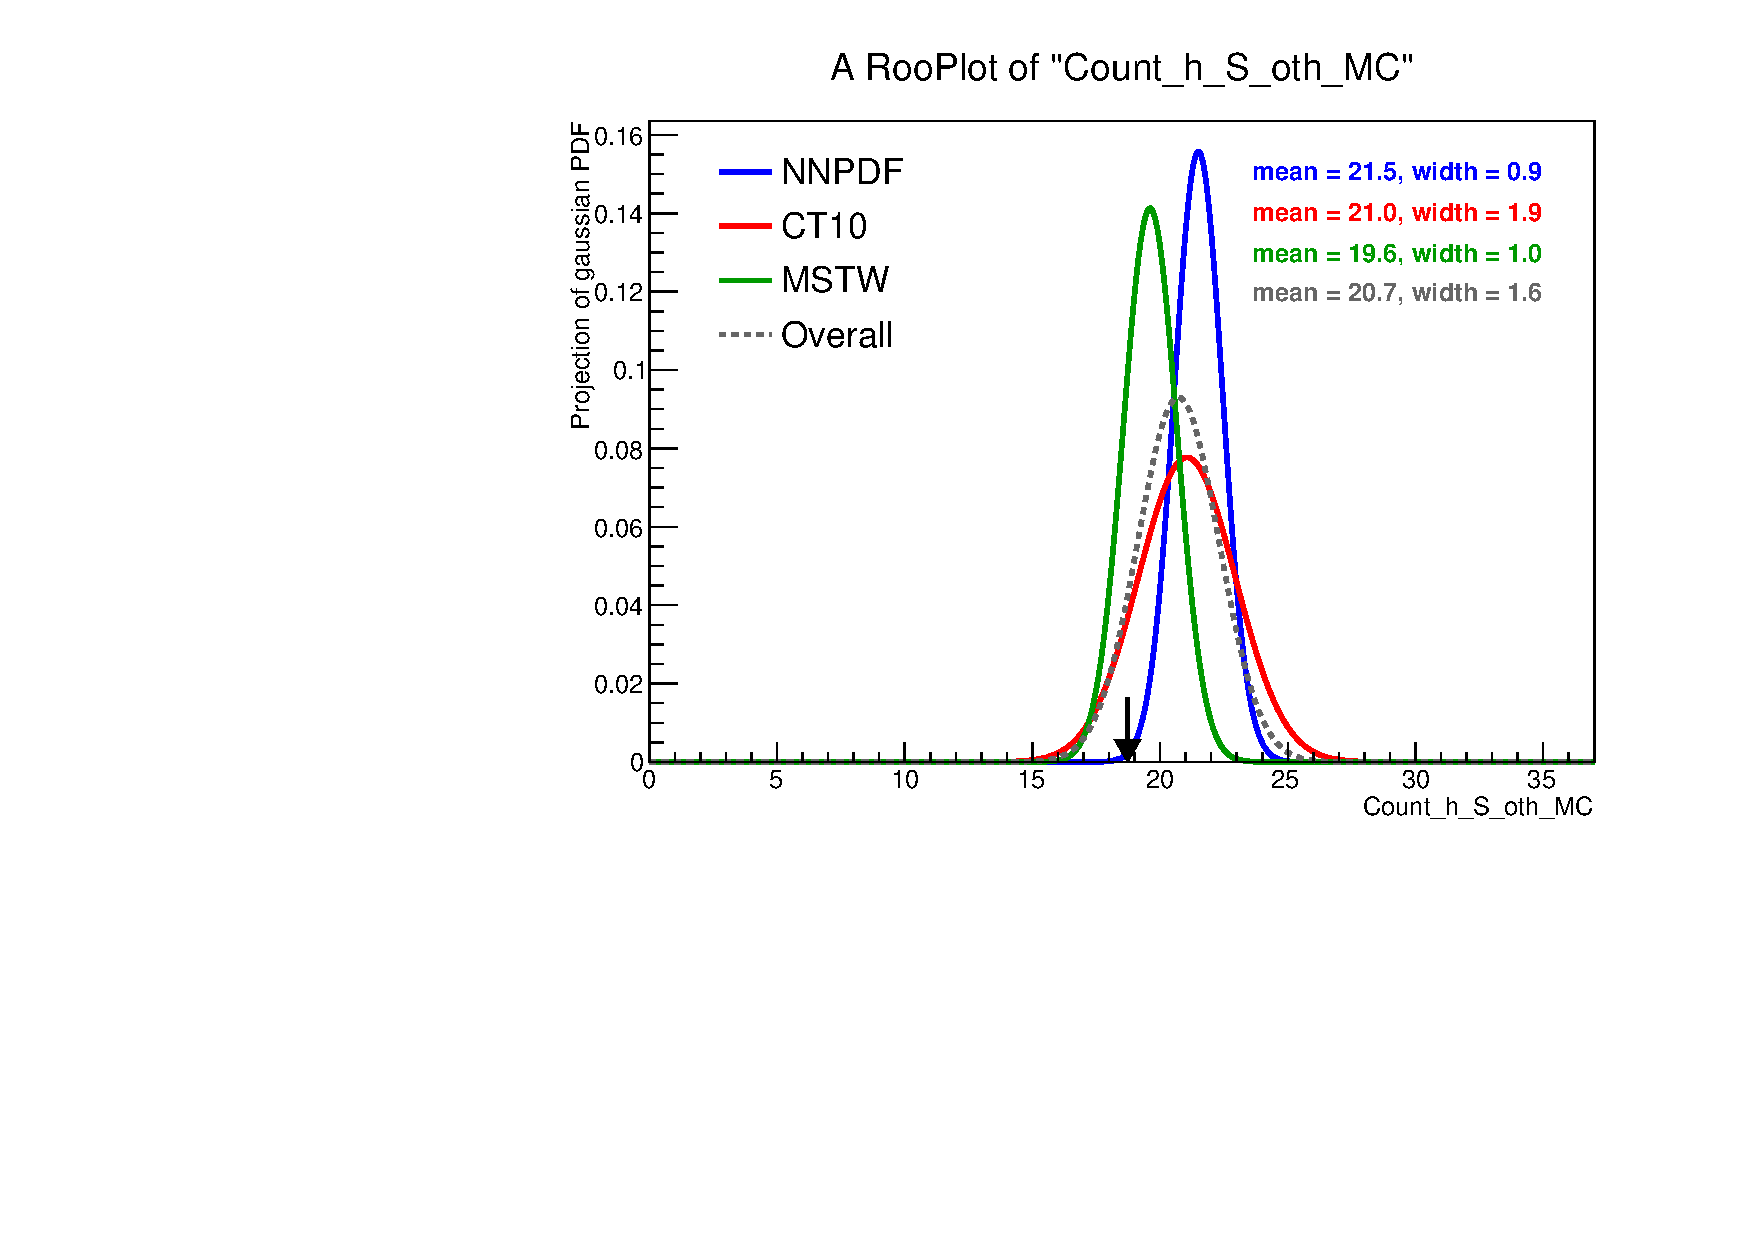
\includegraphics[width=0.48\textwidth,clip=true,trim=0 0.2cm 0 1.2cm]
{figures/razor_systematics/h_S_oth_MC}
~
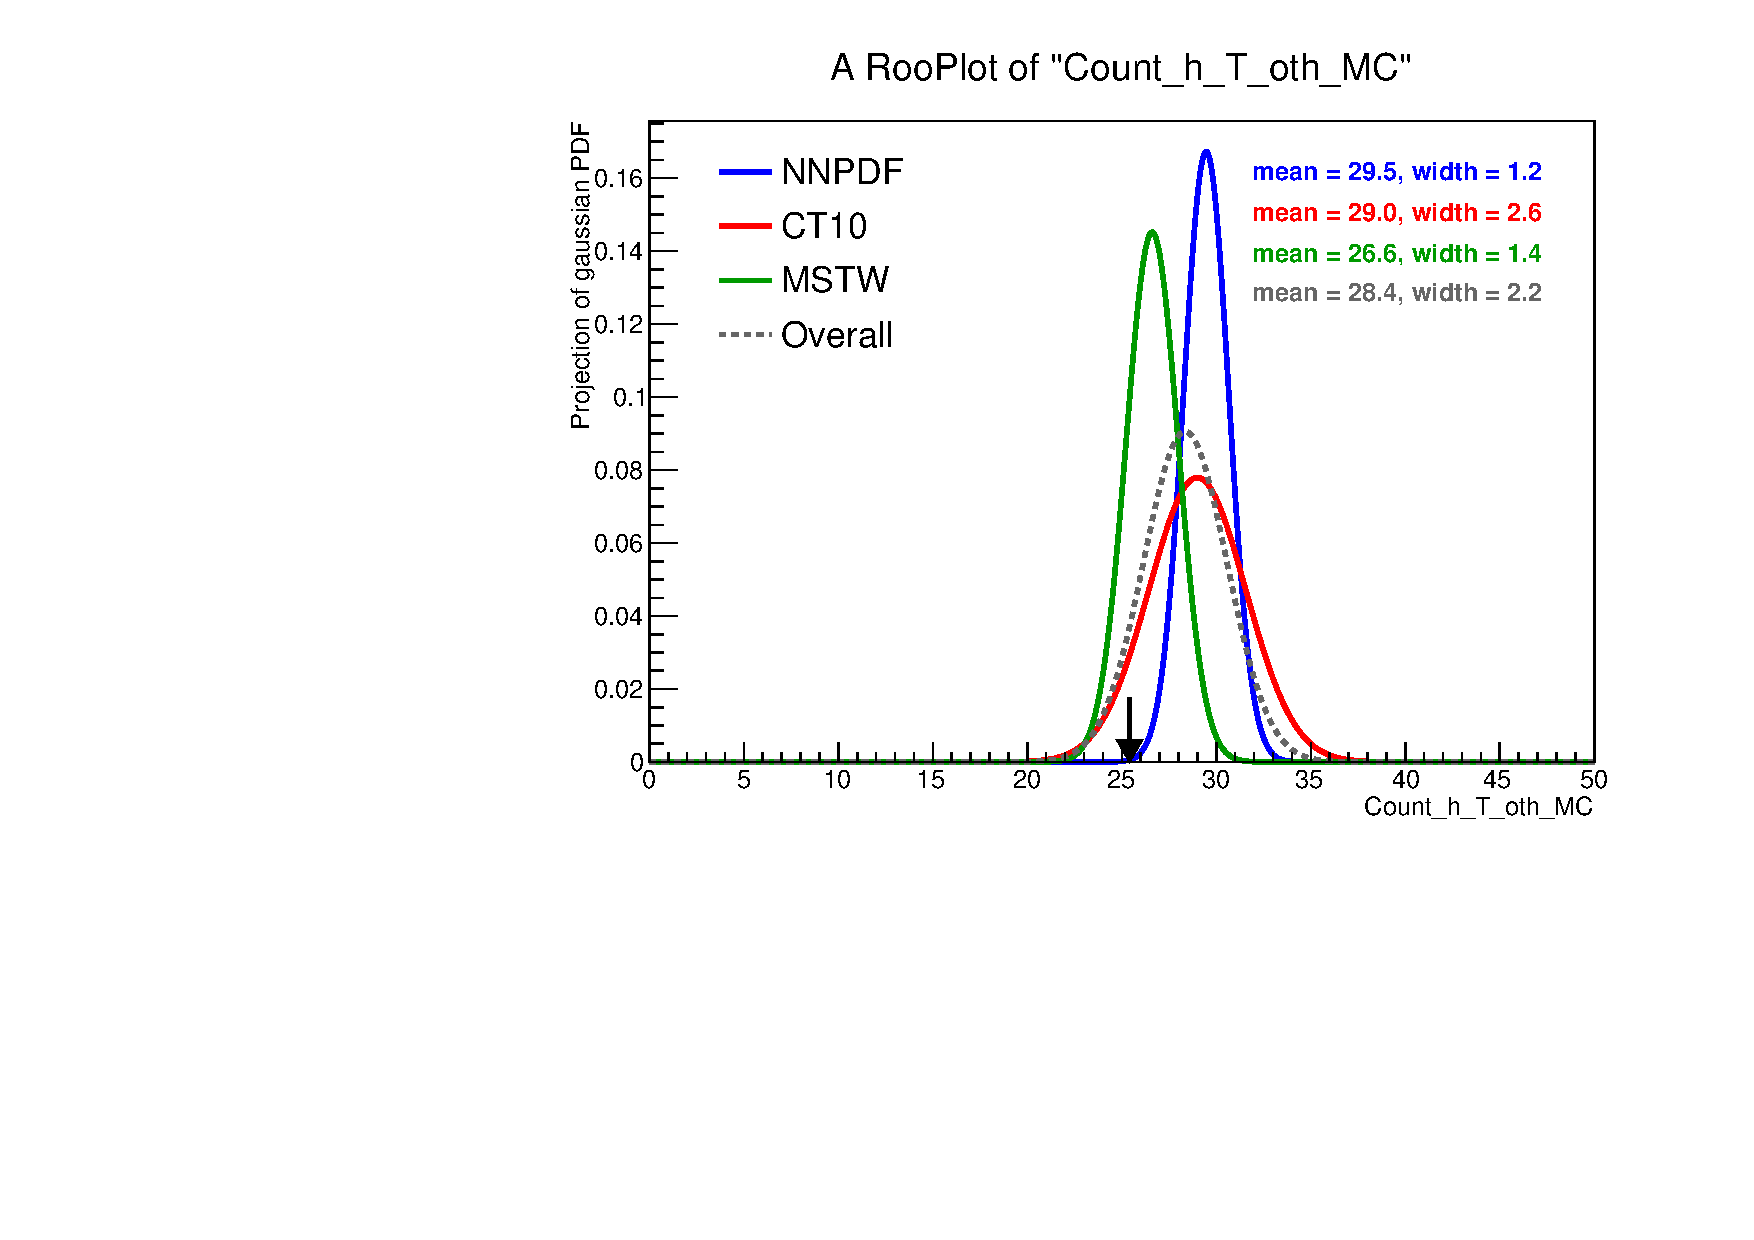
\includegraphics[width=0.48\textwidth,clip=true,trim=0 0.2cm 0 1.2cm]
{figures/razor_systematics/h_T_oth_MC}
\caption{Influence of different PDF sets on the MC counts in the $S$ (left) and $T$ (right) region
for the backgrounds that are taken directly from the simulation.
\label{fig:PDF_effect_on_bg_oth1}}
\end{figure}

\begin{figure}[htpb]
\centering
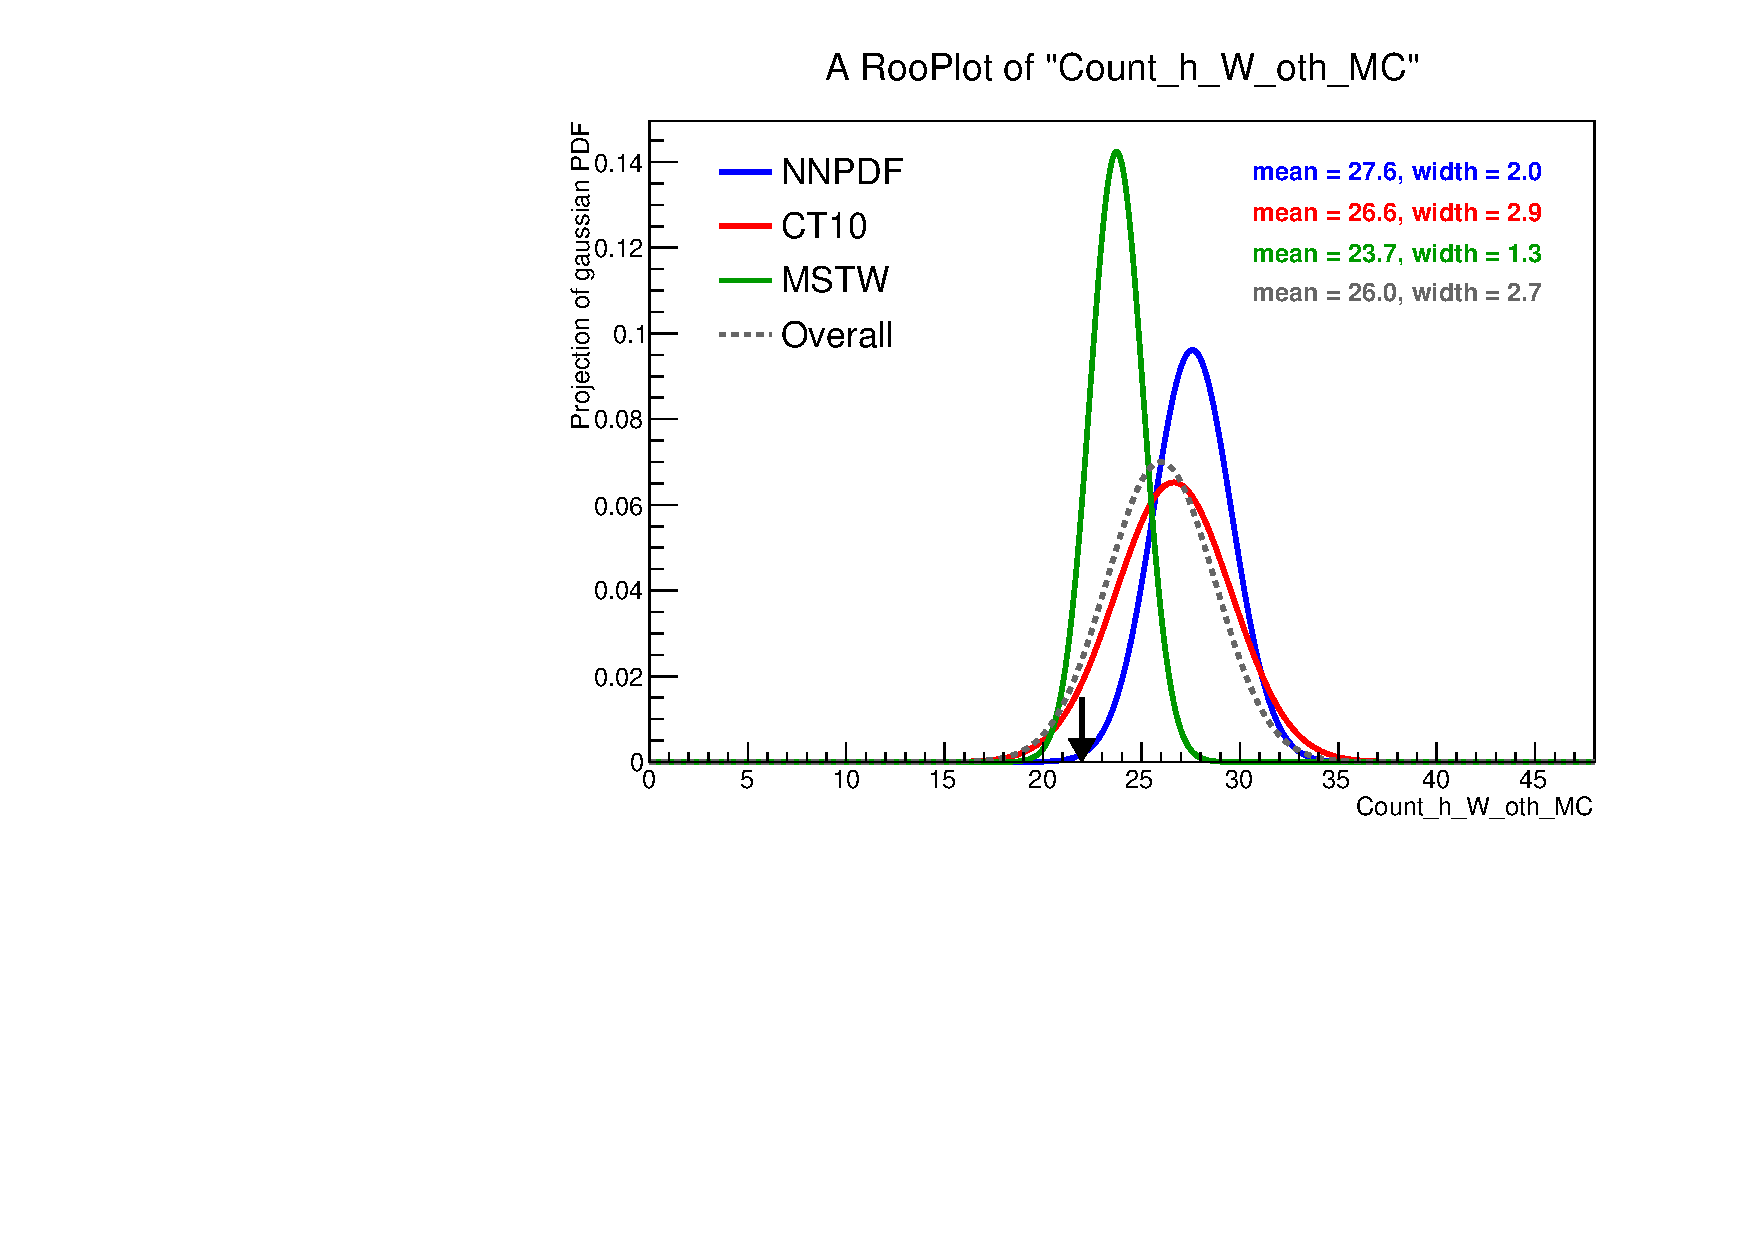
\includegraphics[width=0.48\textwidth,clip=true,trim=0 0.2cm 0 1.2cm]
{figures/razor_systematics/h_W_oth_MC}
~
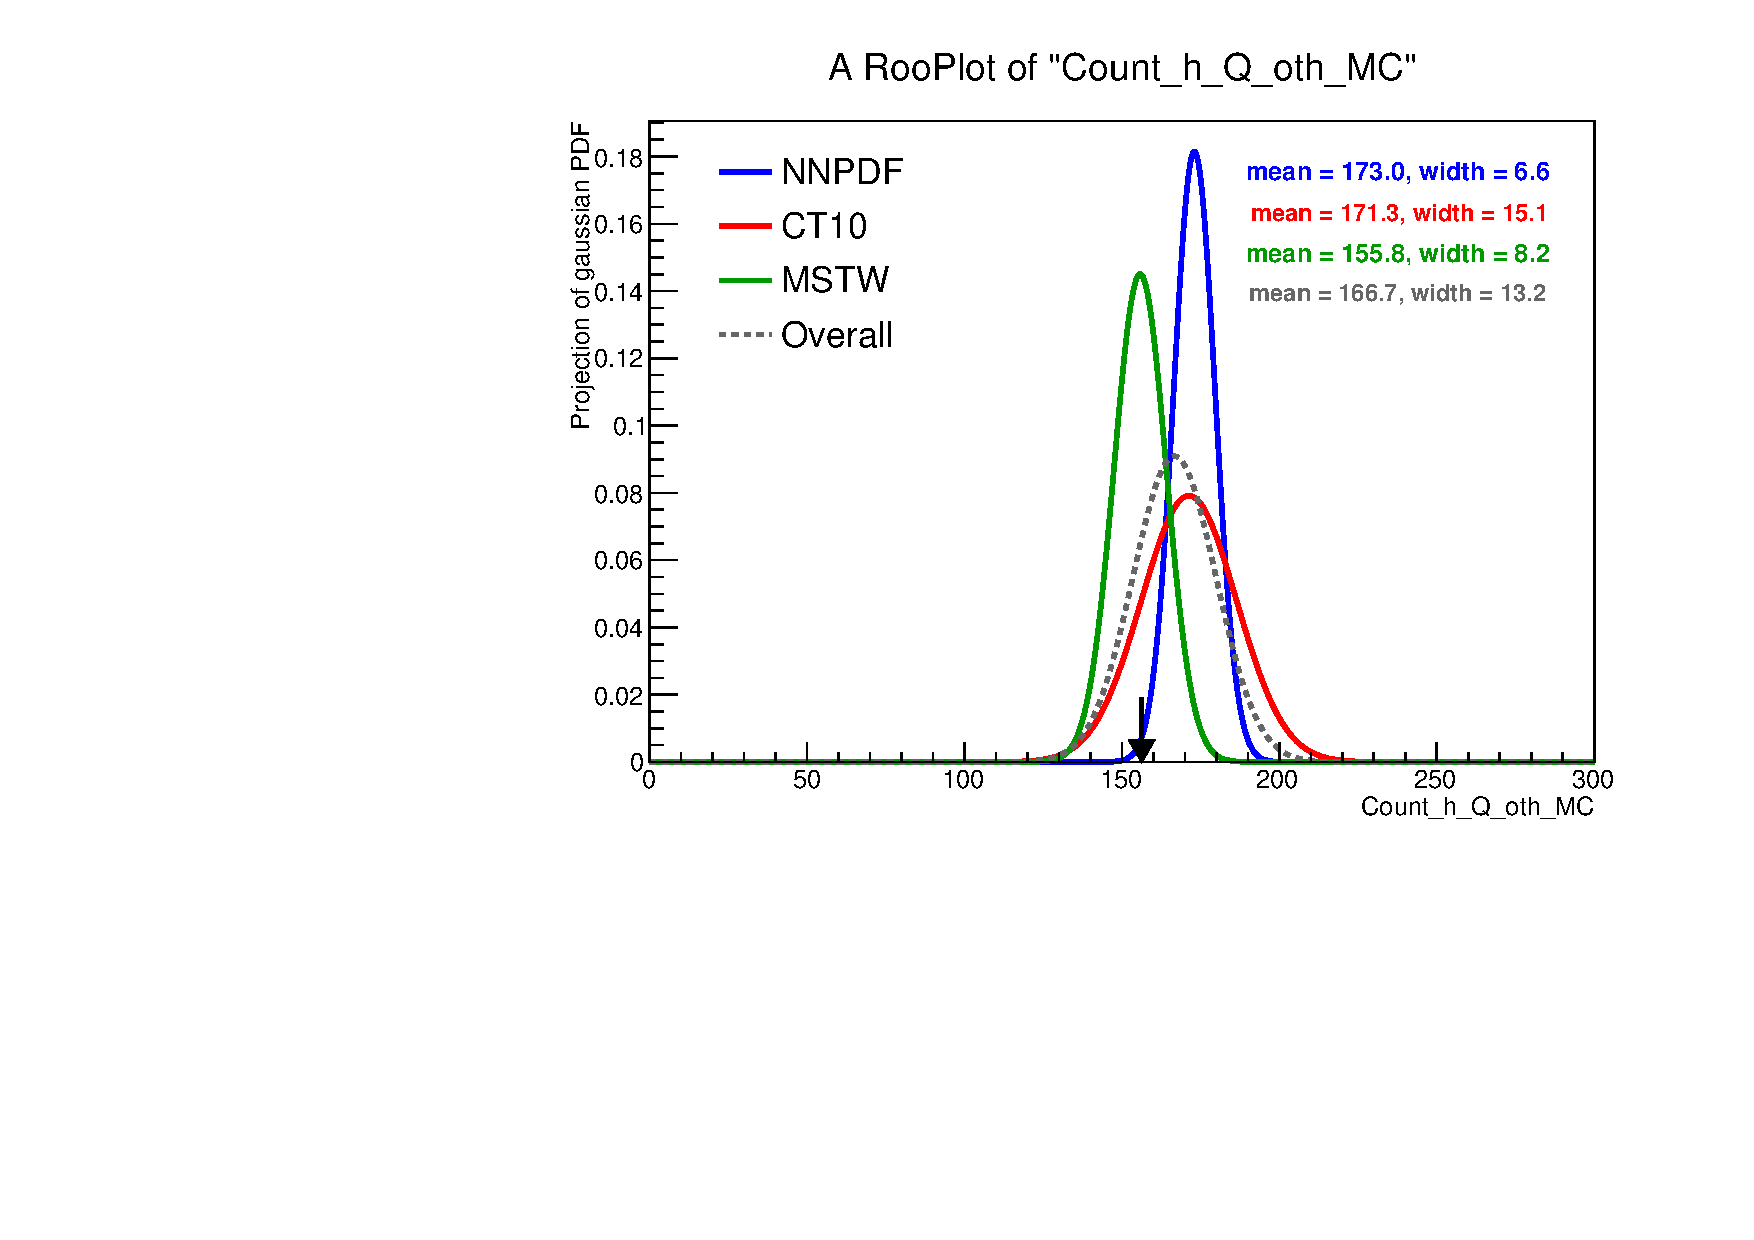
\includegraphics[width=0.48\textwidth,clip=true,trim=0 0.2cm 0 1.2cm]
{figures/razor_systematics/h_Q_oth_MC}
\caption{Influence of different PDF sets on the MC counts in the $W$ (left) and $Q$ (right) region
for the backgrounds that are taken directly from the simulation.
\label{fig:PDF_effect_on_bg_oth2}}
\end{figure}

\begin{figure}[htpb]
\centering
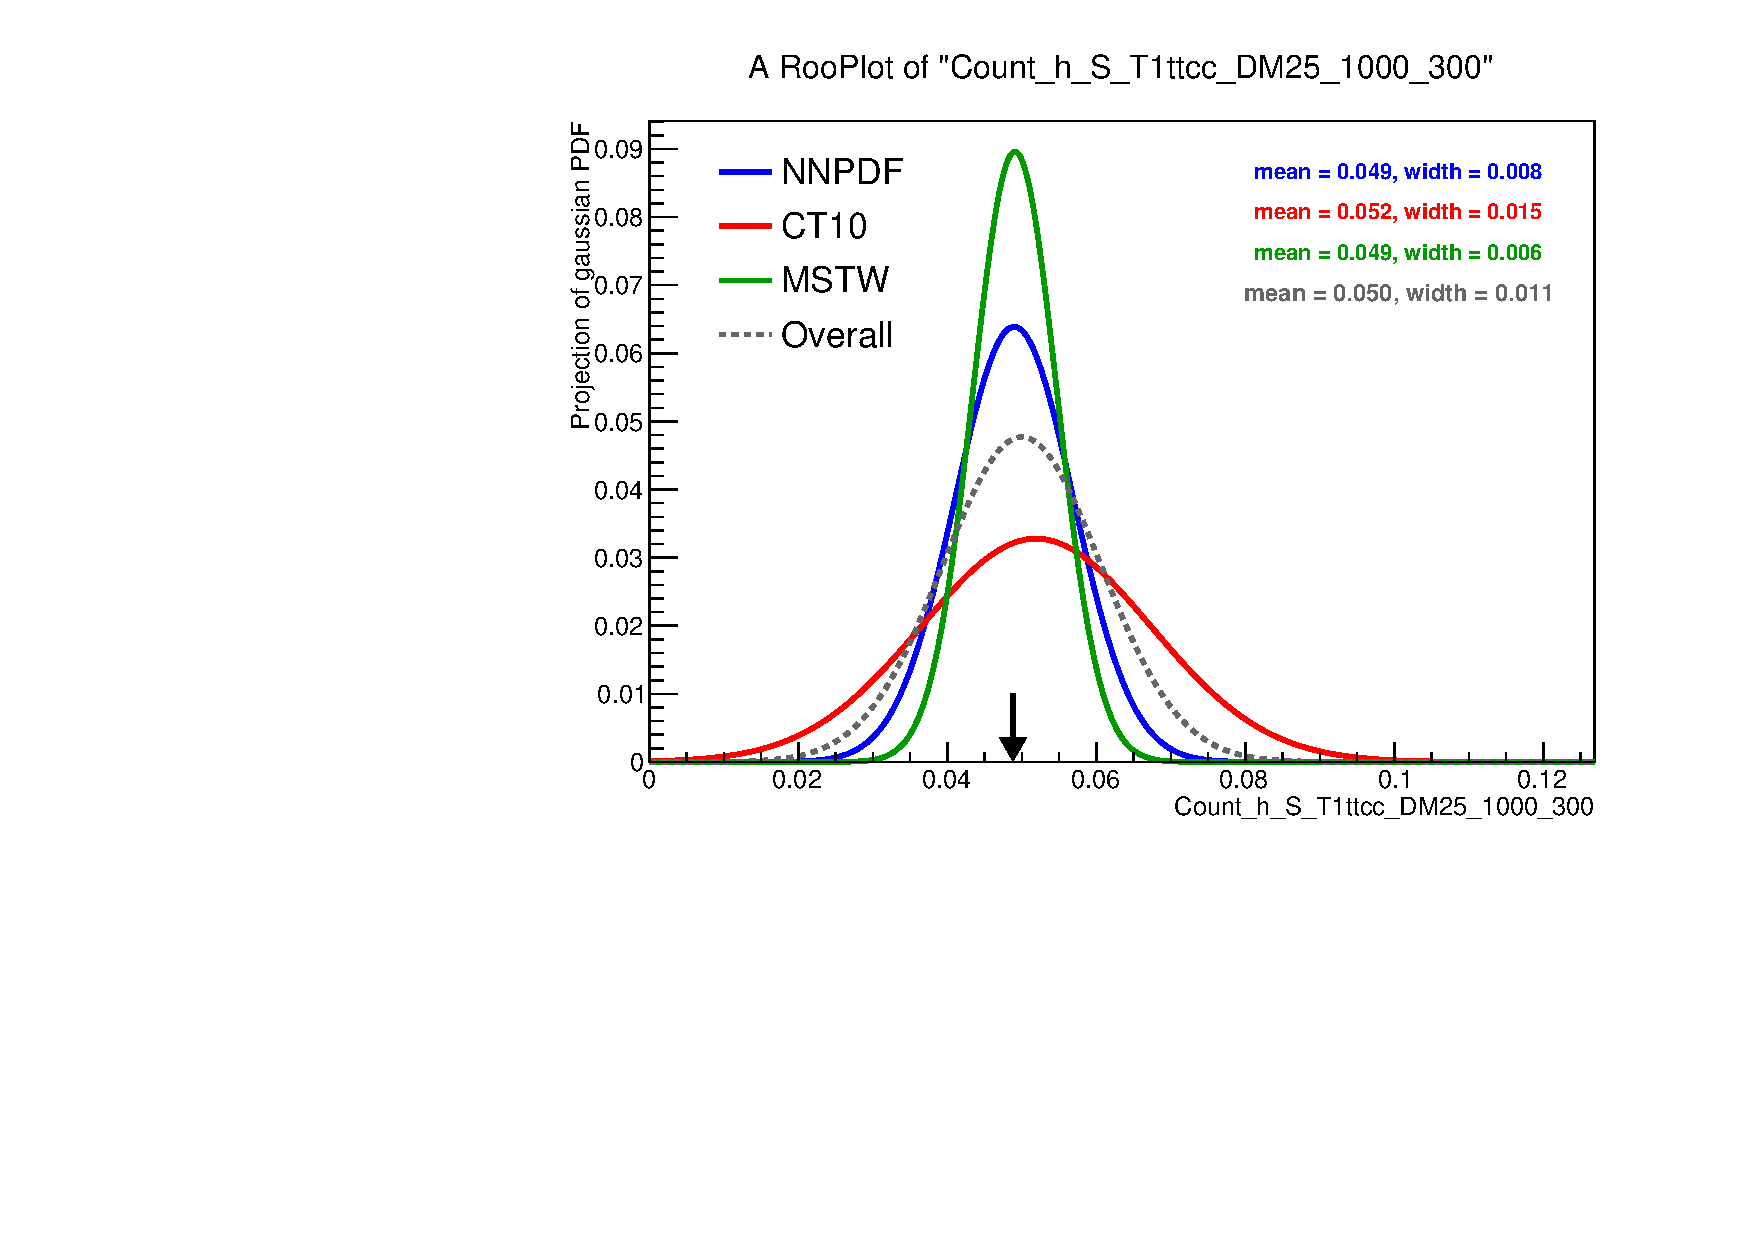
\includegraphics[width=0.48\textwidth,clip=true,trim=0 0.2cm 0 1.2cm]
{figures/razor_systematics/h_S_T1ttcc_DM25_1000_300}
\caption{Influence of different PDF sets on the signal efficiency for the T1ttcc signal point with
$m_{\tilde{g}}=1000\GeV, m_{\tilde{t}_1}=325\GeV, m_{\tilde{\chi}_1^0}=300\GeV$. 
\label{fig:PDF_effect_on_sig}}
\end{figure}

%%%%%%%%%%%%%%%%%%%%%%%%%%%%%%%%%%%%%%%%%%%%%%%%%%%%%%%%%%%%%%%%%%%%%%%%%%%%%%%%%%%%%%%%%%%%%%%%%%%%
\subsection{Trigger efficiency}  

Simulated events are weighted by a trigger efficiency, $\epsilon_{\rm trig}$, according to their
values of $\HT$ and first jet \pt, see Section~\ref{sec:boost_data_trigger}. These trigger weights
have an associated uncertainty coming from the statistical precision of the data samples used to
perform the measurement, and the effect of changing the analysis level selection used to measure the
efficiency. The trigger efficiency uncertainty in each bin, as a function of $\HT$
and leading jet $\pt$, is taken to be the maximum of the statistical uncertainty in the efficiency
after imposing the baseline selection and the difference between the efficiencies before and after
applying the baseline selection. 
Magnitudes of the plus and minus uncertainties, $\delta\epsilon^+_{\rm trig}$ and
$\delta\epsilon^-_{\rm trig}$, were shown in Fig.~\ref{fig:boost_trigger_efficiency_unc}.
The event weight $w_{\rm trig}$ to be applied to the simulated events corresponding to a given
systematic sampling is computed based on the efficiency and uncertainty as follows:
\begin{eqnarray}
w_{\rm trig} & = & \epsilon_{\rm trig}(\HT, \pt^{{\rm j}_1}) + \sigma_{\rm trig}
\delta\epsilon^+_{\rm trig}(\HT, \pt^{{\rm j}_1}), \,\,\, {\rm if} \,\, \sigma_{\rm trig} > 0 \\ 
w_{\rm trig} & = & \epsilon_{\rm trig}(\HT, \pt^{{\rm j}_1}) + \sigma_{\rm trig}
\delta\epsilon^-_{\rm trig}(\HT, \pt^{{\rm j}_1}), \,\,\, {\rm if} \,\, \sigma_{\rm trig} < 0 
\end{eqnarray}
where $\sigma_{\rm trig}$ is the random Gaussian number associated to that particular
systematic sampling.	


%%%%%%%%%%%%%%%%%%%%%%%%%%%%%%%%%%%%%%%%%%%%%%%%%%%%%%%%%%%%%%%%%%%%%%%%%%%%%%%%%%%%%%%%%%%%%%%%%%%%
\subsection{\texorpdfstring{$\cPqb$}{b} tagging \label{sec:boost_btag_sf}} 

The $\cPqb$ tagging performance differs between data and simulation, and differs further between 
CMS FullSim and FastSim.  
The simulated events are therefore corrected by applying data/FullSim and FullSim/FastSim $\cPqb$
tag efficiency scale factors, which depend on the flavour, \pt, and $\eta$ of the jets in the
event. 

There are several methods available to reweight events using the $\cPqb$ tag SFs provided by the CMS
BTAG group~\cite{BTagSF1}. 
Here we choose a method where we consider the number of $\cPqb$ tagged jets in an event to be fixed
to what is given by simulation.  
For a given event, the $\cPqb$-tagging efficiencies for truth $\cPqb$, $\mathrm{c}$ and
$\mathrm{udsg}$ jets, corresponding to the relevant tagging algorithm and working point, are used to
compute the probability that the event has the given $\cPqb$ tagged jet multiplicity. 
We compute $P({\rm sim})$ using efficiencies, $\epsilon^{\rm sim}$, obtained from simulated events,
and we obtain $P(\rm data)$ using efficiencies, $\epsilon^{\rm data}$, that represent data,
\begin{eqnarray}
P(\rm sim) & = & \prod_{i} \epsilon_i^{\rm sim} \prod_{j} (1 - \epsilon_j^{\rm sim}) \\
P(\rm data) & = & \prod_{i} \epsilon_i^{\rm data} \prod_{j} (1 - \epsilon_j^{\rm data})
\end{eqnarray}
where
\begin{equation}
\epsilon^{\rm data} = {\rm SF}^{\rm data}_{\rm sim} \epsilon^{\rm sim} ,
\end{equation}
$i$ runs over the jets that are tagged by the considered $\cPqb$ tagging algorithm, and $j$
runs over the jets that are not tagged.
Our SM MC is simulated with FullSim, so we scale the efficiency with ${\rm SF}^{\rm data}_{\rm sim}
= {\rm SF}^{\rm data}_{\rm Full}$.  
However, the signal samples have been generated using FastSim, so the overall scale factor for
those samples becomes 
${\rm SF}^{\rm data}_{\rm  sim} = {\rm SF}^{\rm data}_{\rm Full} \cdot {\rm SF}^{\rm Full}_{\rm
Fast}$.
The ratio of the two probabilities gives us the weight with which to scale the event,
\begin{equation}
w_{\rm btag} = \frac{P(\rm data)}{P(\rm sim)} .
\end{equation}

The $\cPqb$ tag scale factors have associated uncertainties, $\delta\mathrm{SF}$, which are the
source of the $\cPqb$ tag systematic uncertainty on the background prediction. 
These uncertainties are taken into account in the following way.
$N$ numbers $\sigma_n$ are sampled from a Gaussian with zero mean and unit variance
(different $\sigma$'s are sampled for FullSim and FastSim, and also for different jet truth
flavours). The analysis is then run $N$ times. For each run $n$ we use the corresponding $\sigma_n$
to compute $\epsilon^{\rm data}$ for the FullSim or FastSim samples as follows, 
\begin{align}
\textrm{FullSim: } \epsilon^{\rm data} &= \left(\mathrm{SF^{data}_{Full}} + \sigma_n \, \delta
\mathrm{SF^{data}_{Full}} \right) \cdot \epsilon^{\rm Full} , \\
\textrm{FastSim: } \epsilon^{\rm data} &= \left(\mathrm{SF^{data}_{Full}} + \sigma_n \, \delta
\mathrm{SF^{data}_{Full}}\right) \cdot \left(\mathrm{SF^{Full}_{Fast}} + \sigma_n' \, \delta
\mathrm{SF^{Full}_{Fast}} \right) \cdot \epsilon^{\rm Fast}.
\end{align}
For each of the $N$ runs, $\epsilon^{\rm data}$ will be different, and will lead to a different
event weight $w_{\rm btag}$ such that, overall, the weighted event yields for a given simulated
sample will differ. 
We obtain the systematic uncertainty from the ensemble of the resulting $N$ yields.

In this analysis, we use the CSVM and CSVL $\cPqb$ taggers, see Section~\ref{sec:object_btag}, which
are always used independent of each other. Therefore, for a given event, we compute separate weights
$w_{\rm btag}$ using CSVM and CSVL, and use them only in the relevant regions. The weight obtained
with the CSVM tagger is used in the $S$ and $T$ region, and the CSVL weight in the $W$ and $Q$
region.

%%%%%%%%%%%%%%%%%%%%%%%%%%%%%%%%%%%%%%%%%%%%%%%%%%%%%%%%%%%%%%%%%%%%%%%%%%%%%%%%%%%%%%%%%%%%%%%%%%%%
\subsection{\texorpdfstring{$\W$}{W} tagging} 

The $\W$ boson tag efficiency, and the fake rate for $\W$ boson tag, $\W$ boson mass-tag, and $\W$
boson anti-tag differ between data and simulation, as well as between FullSim and FastSim. 
Data/FullSim and FullSim/FastSim scale factors, whose uncertainties depend on the jet $\pt$,
are applied to the simulated samples to correct for this mismodelling.
Some of these scale factors were derived specifically for this analysis and were described in detail
in Section~\ref{sec:boost_wtag}.
The uncertainties on these scale factors are used in the same way as for the other sources of
systematic uncertainty. For each systematic sampling, the scale factors are varied according to the
sampled uncertainty and propagated to the corresponding event weights.

%%%%%%%%%%%%%%%%%%%%%%%%%%%%%%%%%%%%%%%%%%%%%%%%%%%%%%%%%%%%%%%%%%%%%%%%%%%%%%%%%%%%%%%%%%%%%%%%%%%%
\subsection{Lepton identification \label{sec:boost_leptonID}} 

The razor boost analysis requires the presence of a single loose electron or muon in the definition
of $T$ and $W$ regions. We therefore apply lepton scale factors to our simulated events to correct
for mismodelling of the lepton identification. The uncertainties on these scale factors are
incorporated as a systematic uncertainty on the background prediction.  

For electrons, we use $\pt$ and $\eta$-dependent scale factors and associated uncertainties, as
derived by the CMS EGamma POG~\cite{ElectronSF}.
The overall event weight associated with a given systematic variation of the electron scale
factor, is given as:
\begin{equation}
w_{\rm e} = {\rm SF_{e}}(\pt, \eta) + \sigma_{\rm e} \delta {\rm SF_{e}}(\pt, \eta), 
\end{equation}
where $\sigma_{\rm e}$ is the random Gaussian number associated with the given systematic variation.
The scale factors for muons are approximately equal to unity, with negligible uncertainties. Their
variation is, consequently, not taken into account.

%%%%%%%%%%%%%%%%%%%%%%%%%%%%%%%%%%%%%%%%%%%%%%%%%%%%%%%%%%%%%%%%%%%%%%%%%%%%%%%%%%%%%%%%%%%%%%%%%%%%
\subsection{Initial State Radiation} 

Deficiencies in the modelling of initial state radiation are corrected by reweighting the
signal samples using an event weight that depends on the \pt of the recoiling system, which in this
case is the $\tilde{g}\tilde{g}$ system. 
More information on this reweighting and how it was derived, was given in
Section~\ref{sec:event_ISRreweighting}. 
The associated uncertainty on the ISR reweighting, see Table~\ref{tab:ISRreweighting} for the
numerical values, is incorporated as a systematic uncertainty on the signal efficiency. 

%%%%%%%%%%%%%%%%%%%%%%%%%%%%%%%%%%%%%%%%%%%%%%%%%%%%%%%%%%%%%%%%%%%%%%%%%%%%%%%%%%%%%%%%%%%%%%%%%%%%
\subsection{Top quark \texorpdfstring{\pt}{pT} spectrum} 

Differential top-quark-pair cross section analyses have shown that the shape of the \pt spectrum of 
top quarks in data is softer than predicted by simulation. 
To account for this, we reweight events based on the \pt of the generator level $t$ and $\bar{t}$
quarks in the $t\bar{t}$ simulation, as explained in Section~\ref{sec:event_toppt_reweighting}. 
The uncertainty associated with this reweighting is equal to the full size of the
reweighting, and is propagated as a systematic uncertainty to the final background estimation. 

%%%%%%%%%%%%%%%%%%%%%%%%%%%%%%%%%%%%%%%%%%%%%%%%%%%%%%%%%%%%%%%%%%%%%%%%%%%%%%%%%%%%%%%%%%%%%%%%%%%%
\subsection{Pileup} 

Simulated events are reweighted such that their pileup distribution matches the observed pileup
distribution, see Section~\ref{sec:event_pileup}. The uncertainty on this procedure is largely
driven by the uncertainty on the minbias cross section. We consider a variation in the minbias cross
section of $\pm 5\%$, thereby changing the shape of observed pileup distribution and
therefore the resulting pileup event weights. The difference in weights is taken as a measure of the
uncertainty in the pileup distribution, and is multiplied by the random number, $\sigma_{\rm PU}$,
associated to each given sampling.  The pileup weight that is applied in each sampling is given by
\begin{eqnarray}
w_{\rm PU} & = & w_{\rm PU}^{\rm nom} + \sigma_{\rm PU}\delta w^+_{\rm PU}, \,\,\, {\rm if}
\,\, \sigma_{\rm PU} > 0, \\ 
w_{\rm PU} & = & w_{\rm PU}^{\rm nom} + \sigma_{\rm PU}\delta w^-_{\rm PU}, \,\,\, {\rm if}
\,\, \sigma_{\rm PU} < 0. 
\end{eqnarray}
with $w_{\rm PU}^{\rm nom}$ the nominal pileup weight, $\delta w^+_{\rm PU} = w_{\rm PU}^{+5\%} -
w_{\rm PU}^{\rm nom}$, and $\delta w^-_{\rm PU} = w_{\rm PU}^{\rm nom} - w_{\rm PU}^{-5\%}$.

%%%%%%%%%%%%%%%%%%%%%%%%%%%%%%%%%%%%%%%%%%%%%%%%%%%%%%%%%%%%%%%%%%%%%%%%%%%%%%%%%%%%%%%%%%%%%%%%%%%%
\subsection{QCD spectrum} 

The closure tests described in Section~\ref{sec:boost_closure_tests} showed that there is a 40\%
uncertainty in the QCD multijet scale factor $\kappa_{\rm QCD}^{Q/S}$ between the signal and $Q$
regions. 
A quantitative verification of this number is given in the next paragraph. 
The uncertainty is accounted for in the background prediction method by including an additional 33\%
uncertainty directly on the $\kappa_{\rm QCD}^{Q/S}$ parameter, as was mentioned in
Section~\ref{sec:boost_likelihood}.
This is the only systematic uncertainty treated in this way. Every other systematic uncertainty is
dealt with during the systematic sampling from which the expected simulated counts are computed.

The level of closure in the second cross check, see Section~\ref{sec:boost_closure_tests}, can be
computed using the ratio between observed data and prediction.
We model each bin of that ratio, on the two-dimensional (\mr, \rsq) plane, as a Gaussian
distribution, with the uncertainty on the ratio for that bin as the width of the Gaussian. 
We scale each distribution to the number of observed events, thus giving more weight to bins with
higher precision, and finally sum over all of them. 
From this total distribution we then compute the interval around unity that contains approximately
68\% of the integral. 
This procedure is illustrated in Fig.~\ref{fig:boost_systematics_closure_QCD}. 
On the left the ratio data/prediction with associated statistical uncertainty is shown for each bin
in the two-dimensional razor space. 
On the right-hand side we show the Gaussian distributions and the corresponding 68\% interval that
constitutes the total systematic uncertainty, 40\%, that needs to be applied. 

\begin{figure}[htpb]
\centering
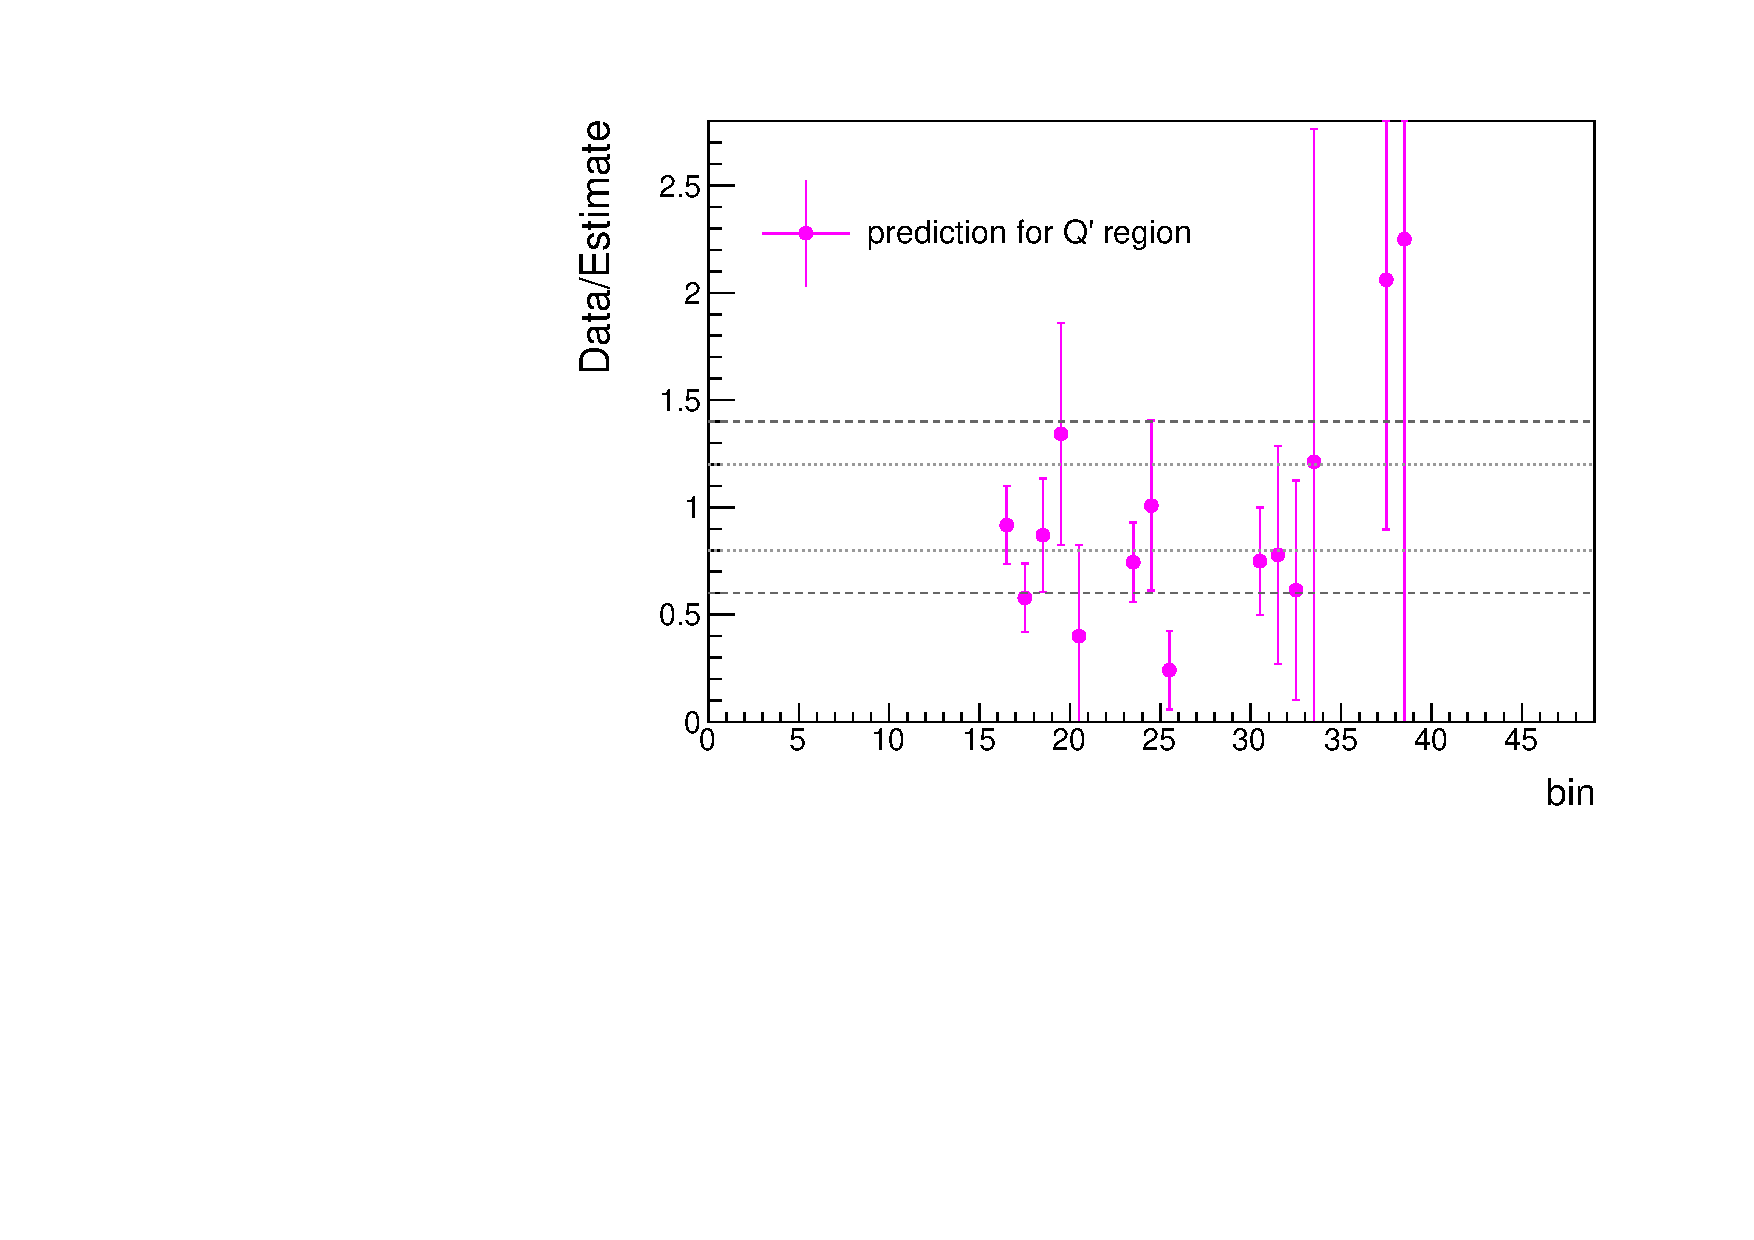
\includegraphics[width=0.48\textwidth]{figures/razor_systematics/closure_summary_0p5_magenta}
~
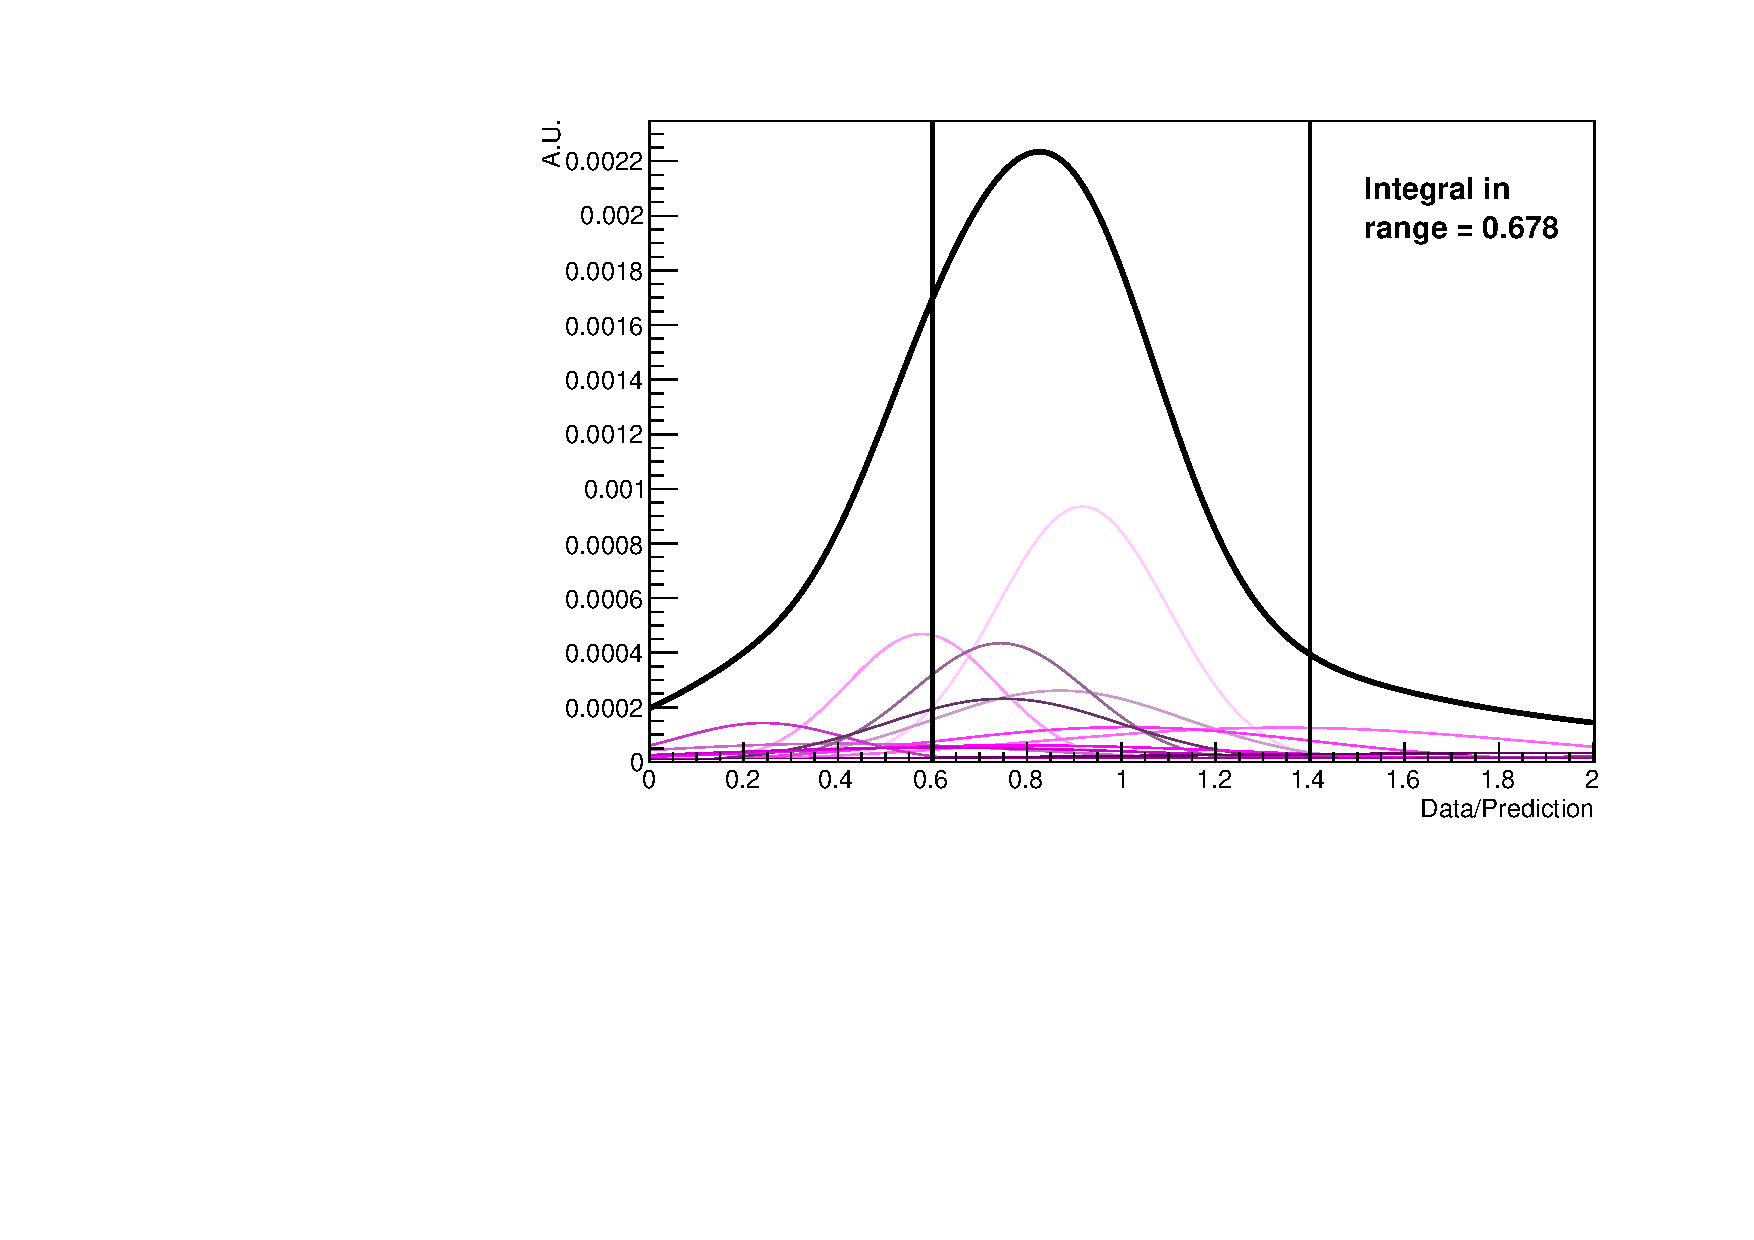
\includegraphics[width=0.48\textwidth]{figures/razor_systematics/closure_summary_0p5_magenta_gauss2}
\caption{[left] Data/prediction for each of the 25 bins in the 2D $(\mr, \rsq)$ plane for the
closure test predicting the background in region $Q'$. Uncertainties are statistical only.
[right] We represent the agreement between data and prediction for the closure test predicting the
background in region $Q'$ as a Gaussian probability density function for each bin in the 2D
$(\mr,\rsq)$ plane. Each bin is shown as a Gaussian in a different shade of magenta. The sum of all
Gaussians is depicted in black. Each separate component has been normalized to the weight it
carries in the sum. 
\label{fig:boost_systematics_closure_QCD}}
\end{figure}

%%%%%%%%%%%%%%%%%%%%%%%%%%%%%%%%%%%%%%%%%%%%%%%%%%%%%%%%%%%%%%%%%%%%%%%%%%%%%%%%%%%%%%%%%%%%%%%%%%%%
\subsection{\texorpdfstring{$\cPZ (\rightarrow \nu \bar{\nu})+$jets}{Z(nunu)+jets} in
association with heavy flavour} 

About 8\% of the background in the signal region is composed of
$\cPZ({\rightarrow}\,\nu\bar{\nu})$+jets
events. Since we require the presence of at least one $\cPqb$ tagged jet, and given the known
deficiency in modelling $\cPZ$ production in association with heavy flavour, we include an extra
systematic uncertainty in the $\cPZ({\rightarrow}\,\nu\bar{\nu})$+jets contribution.  

This uncertainty is estimated using a data control region enriched in
$\cPZ({\rightarrow}\, \ell \bar{\ell})+$jets, required, in addition to the baseline selection
requirements, to contain exactly two tight leptons ($e$ or $\mu$), of same flavour and opposite
sign, with dilepton invariant mass consistent with the $\cPZ$ boson mass, $60 < m_{\ell\bar{\ell}} <
120\GeV$.
We also require the presence of at least one $\cPqb$ tagged jet, and at least one $\W$
boson mass-tagged jet.  A comparison between data and simulation in this $\cPZ$-enriched control
region is presented in Fig.~\ref{fig:DataMC_ZCR}. The simulation is seen to overpredict the data. 

We estimate the systematic uncertainty in the $\cPZ({\rightarrow}\,\nu\bar{\nu})$+jets contribution
by first computing bin-by-bin data/simulation ratios, on the ($\mr,\rsq$) space, in this control
region. Then, we take the statistical uncertainty in the ratio for each bin as the
standard deviation of a Gaussian distribution, normalized to the number of events in that bin.  
Finally, the Gaussians from all bins are superposed, and the total uncertainty is taken to be the
magnitude of the 68\% band around a ratio of unity. 
Figure~\ref{fig:boost_systematics_Zinv} illustrates this procedure, showing the bin-by-bin ratios
and the superposed Gaussians.
Based on these results, we decide to put an additional uncertainty of 50\% on the contribution of 
$Z({\rightarrow}\,\nu\bar{\nu})$ in association with heavy flavour. 

\begin{figure}[htpb]
\centering
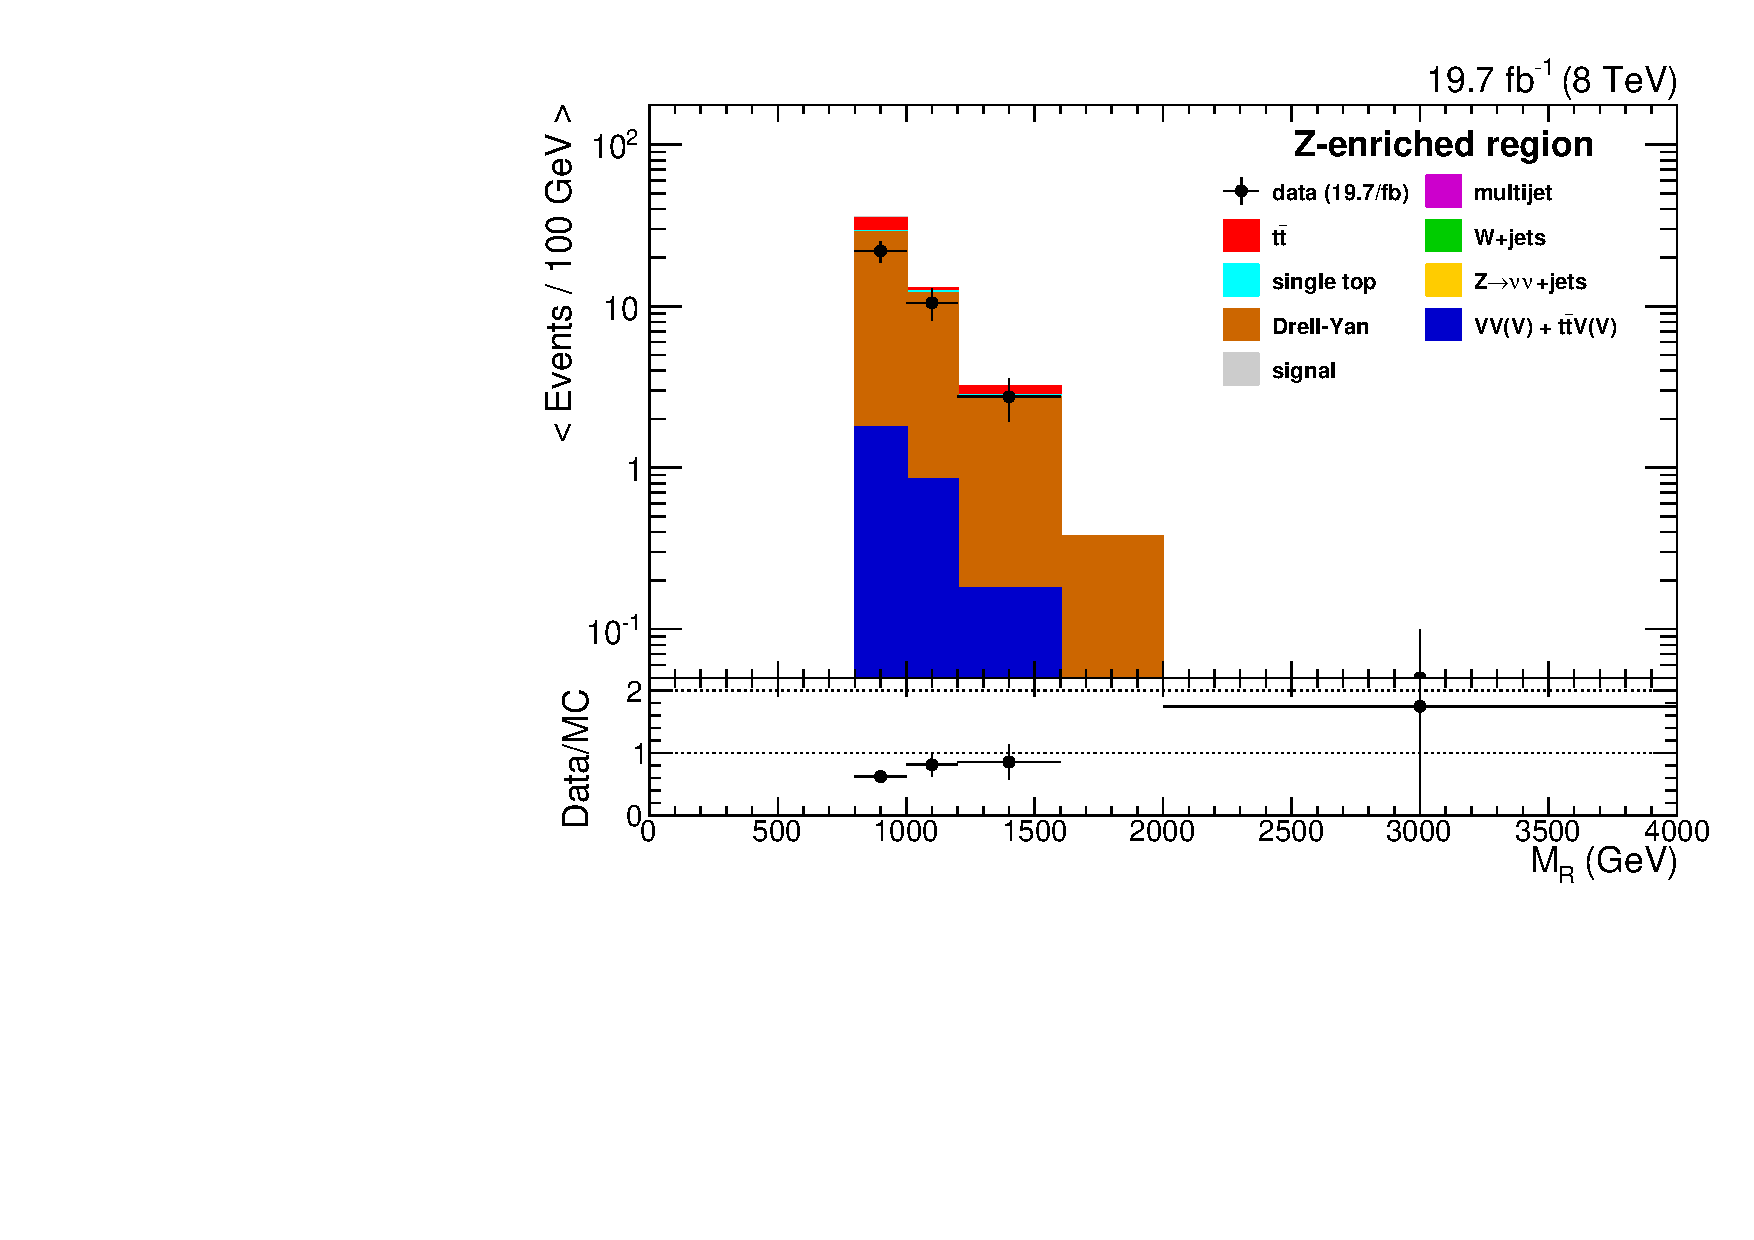
\includegraphics[width=0.48\textwidth]{figures/razor_selection/plots/DataMC_MR_g1Mbg1Y2l0ol_width}
~
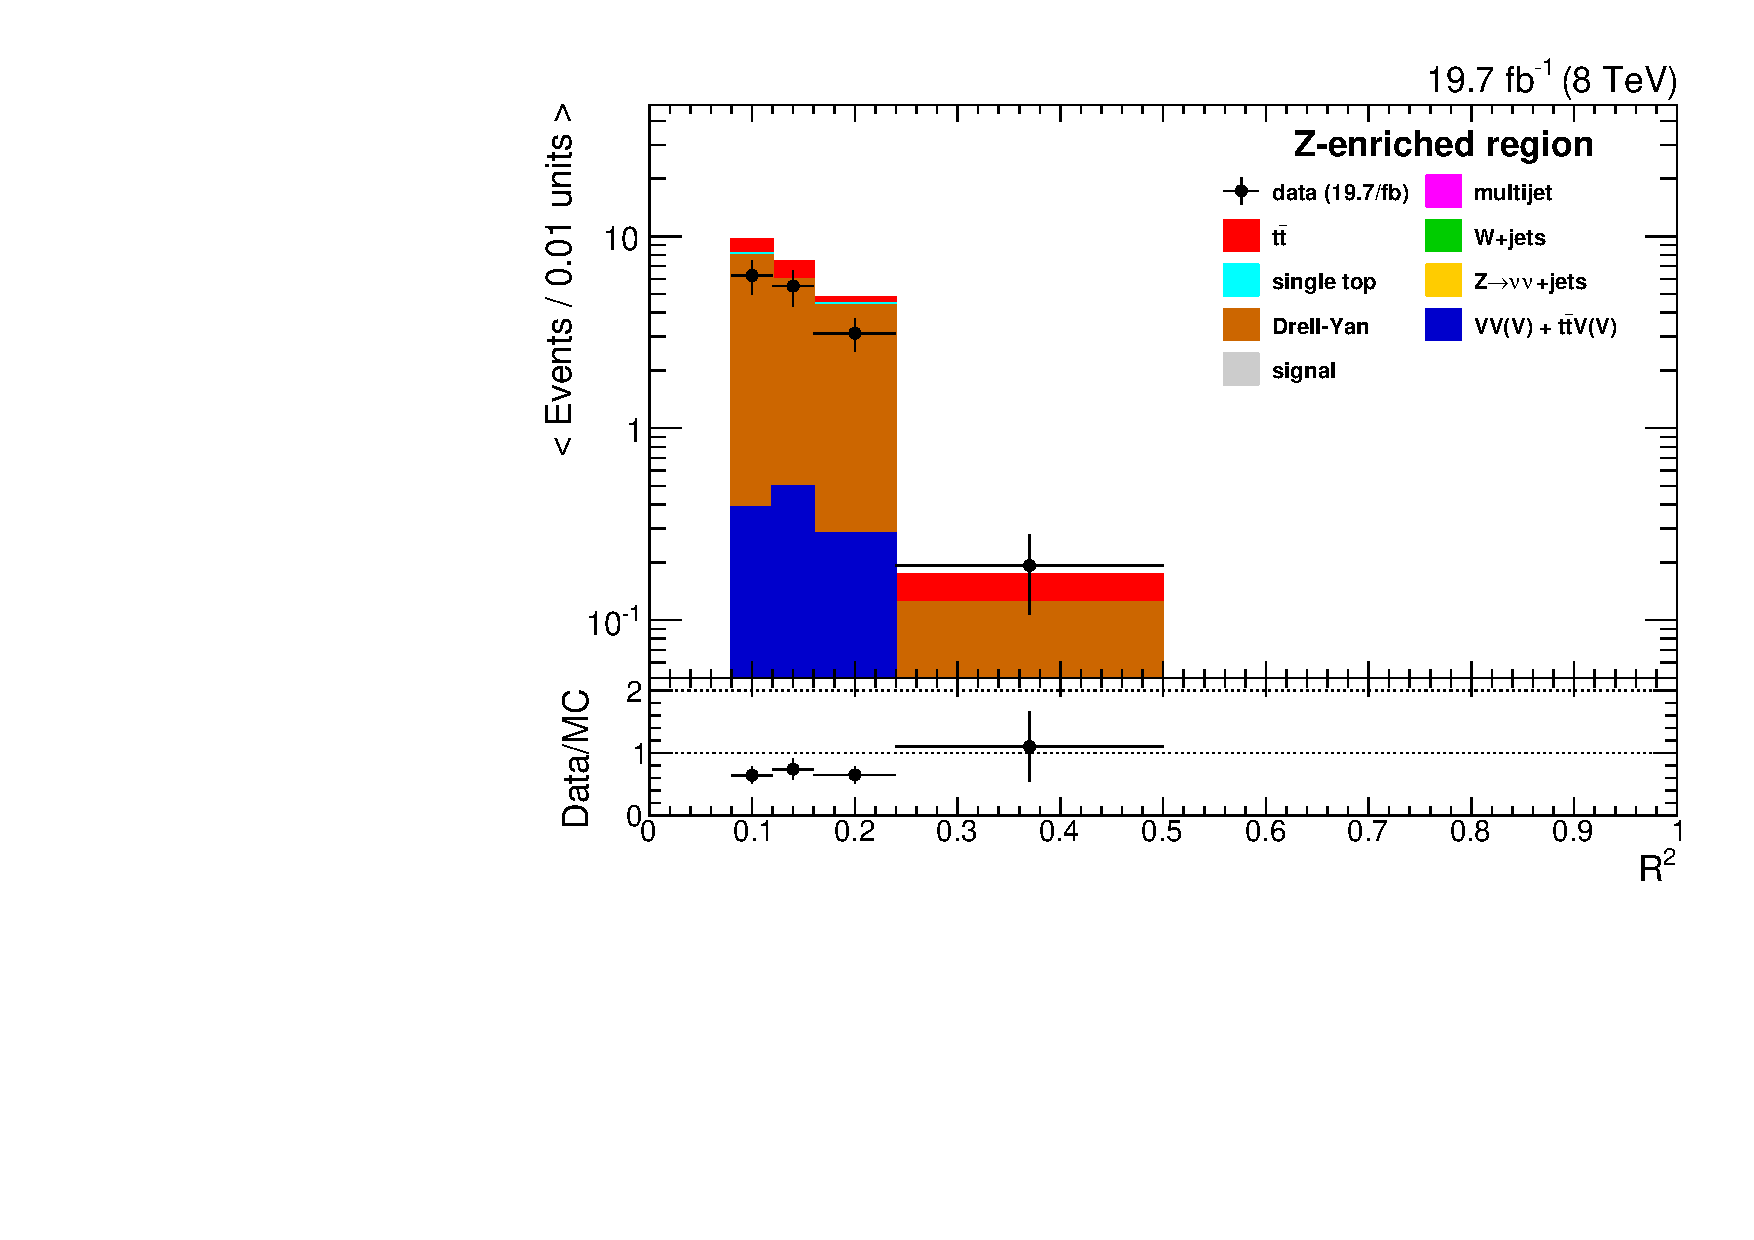
\includegraphics[width=0.48\textwidth]{figures/razor_selection/plots/DataMC_R2_g1Mbg1Y2l0ol_width}
\caption{Comparison of data and simulation for the $\mr$ (left) and $\rsq$ (right) distributions in
the $\cPZ\rightarrow \ell \bar{\ell}$ control region with at least one $\cPqb$ tagged jet and at
least one mass-tagged $\W$ boson candidate. 
\label{fig:DataMC_ZCR}}
\end{figure}

\begin{figure}[htpb]
\centering
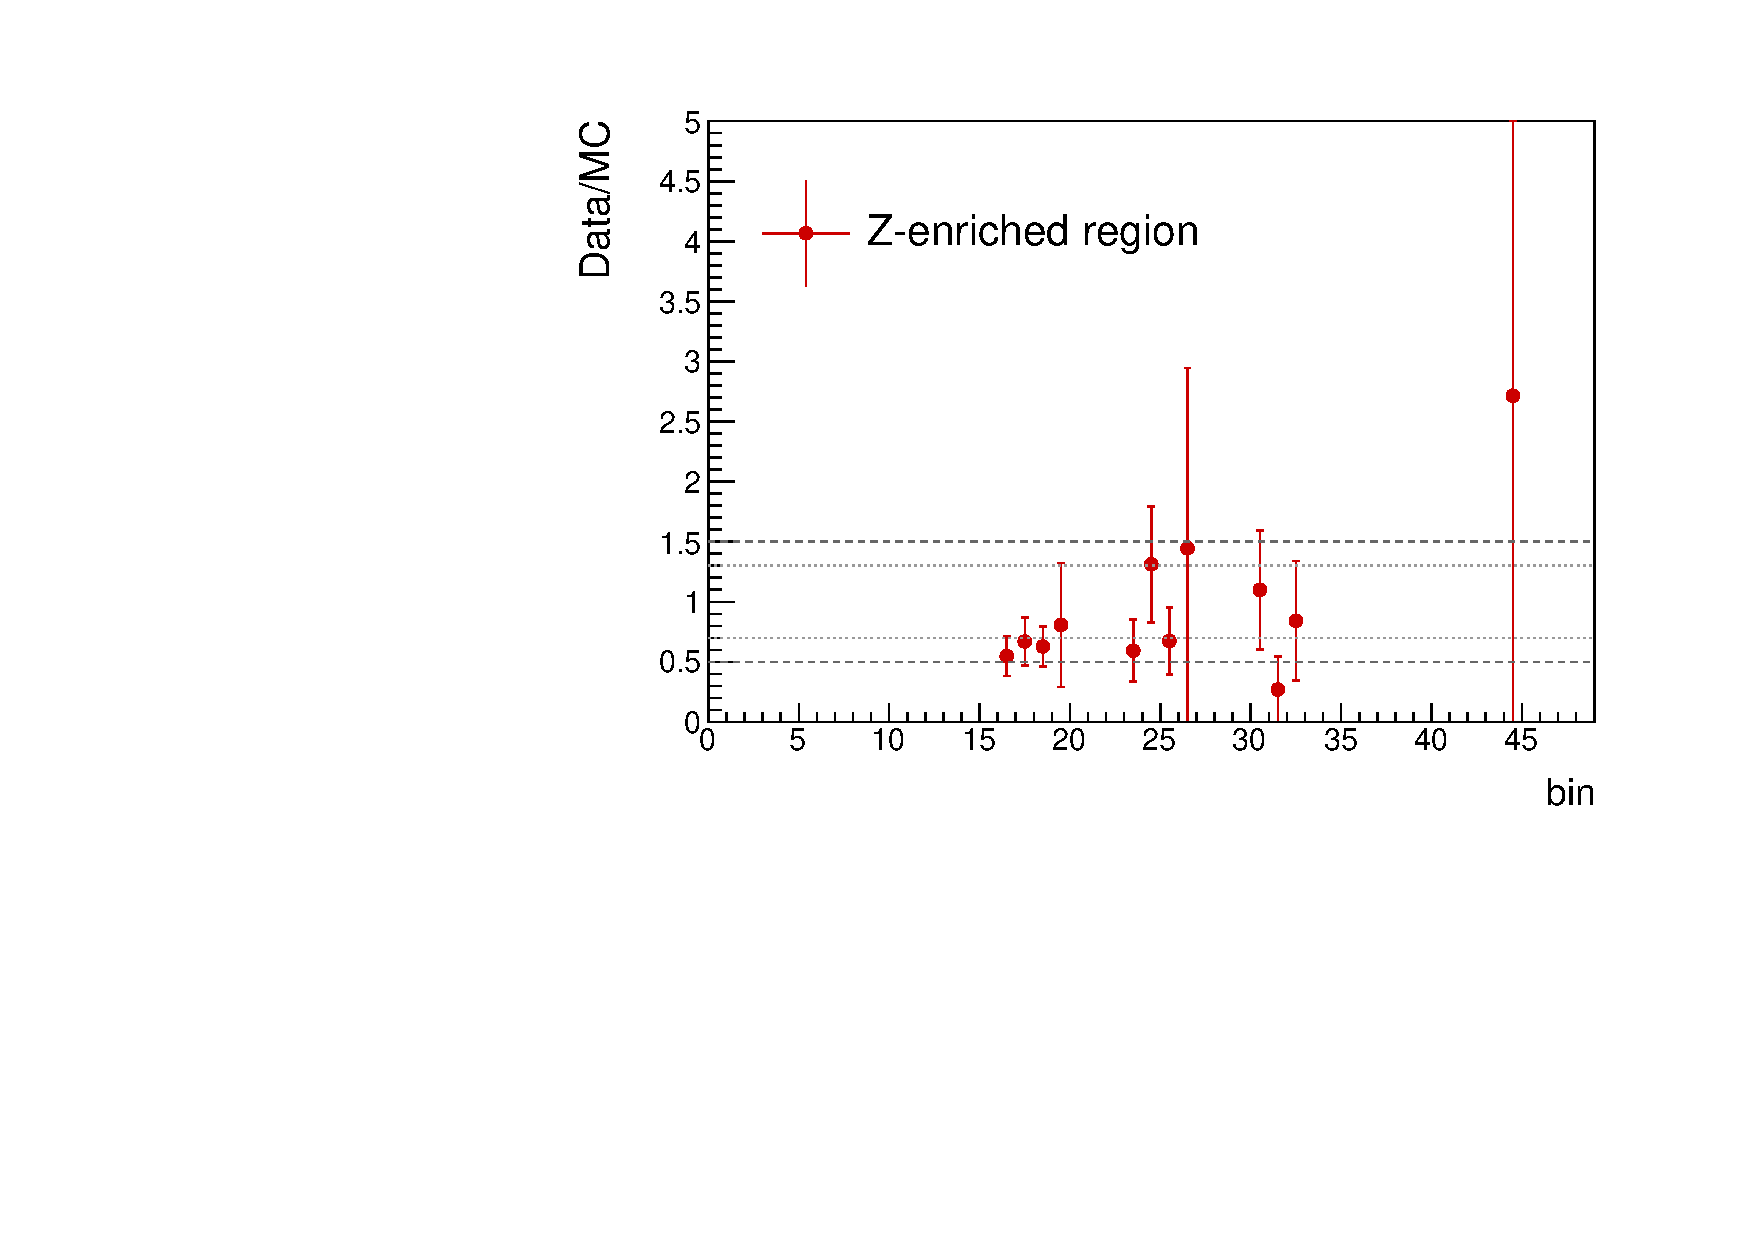
\includegraphics[width=0.48\textwidth,clip=true,trim=0 0.5cm 0.5cm 1.2cm]
{figures/razor_systematics/Data_MC_1D_g1Mbg1Y2l0ol}
~
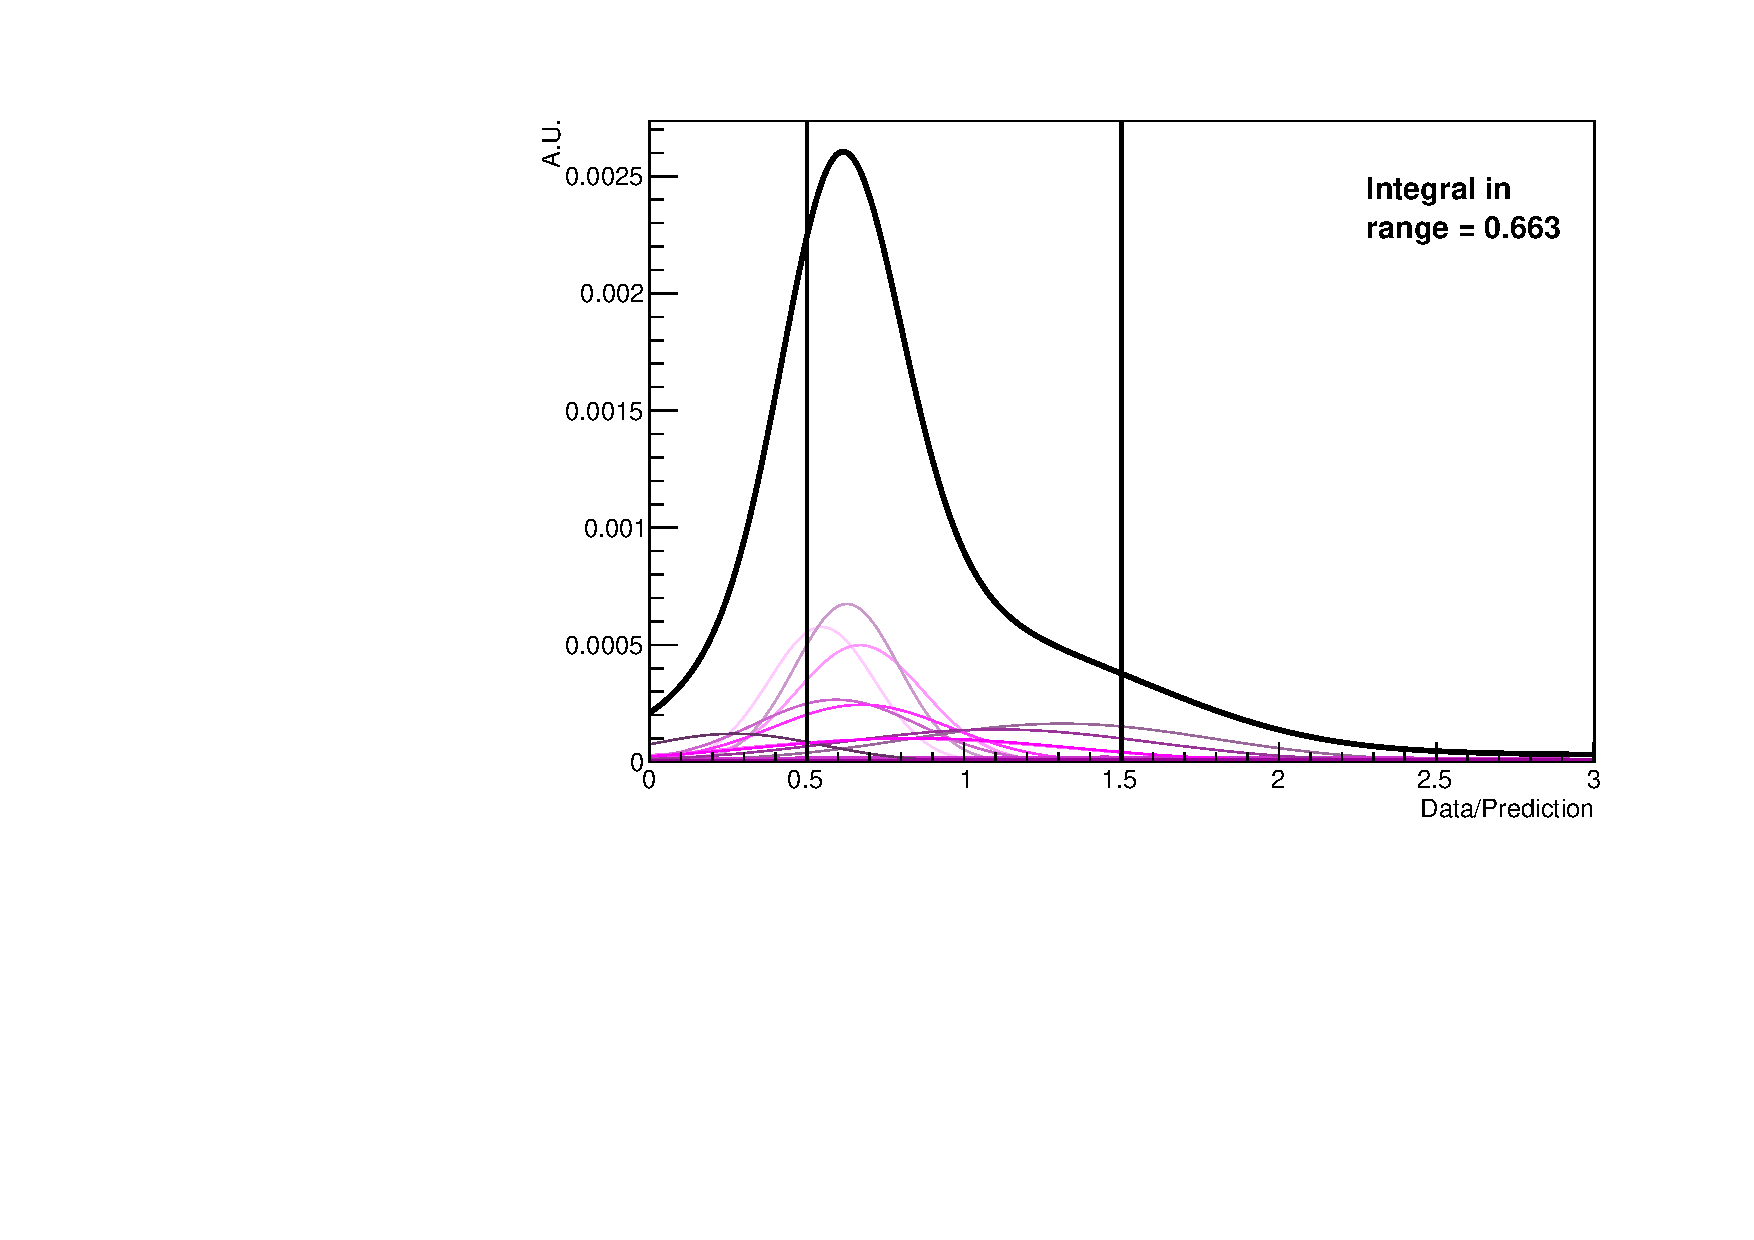
\includegraphics[width=0.48\textwidth]{figures/razor_systematics/Zinv_g1Mbg1Y2l0ol2}
\caption{[left] Ratio data/simulation for each bin in the 2D ($\mr,\rsq$) plane for the
$\cPZ$-enriched control region mentioned in the text. Uncertainties are statistical only.
[right] We represent the agreement between data and simulation for the $\cPZ$-enriched control
region as a Gaussian probability density function for each bin in the 2D ($\mr,\rsq$) plane. Each
bin is shown as a Gaussian in a different shade of magenta. The sum of all Gaussians is
depicted in black. Each separate component is normalized to the weight it carries in the sum. 
\label{fig:boost_systematics_Zinv}}
\end{figure}


%%%%%%%%%%%%%%%%%%%%%%%%%%%%%%%%%%%%%%%%%%%%%%%%%%%%%%%%%%%%%%%%%%%%%%%%%%%%%%%%%%%%%%%%%%%%%%%%%%%%
\subsection{Summary of separate systematic effects}

As noted before, all systematic effects are varied simultaneously. However, in order to see the
effect of each systematic uncertainty individually, each systematic effect $i$ is varied by one
standard deviation up and down.  
The effect on the background and signal samples in the signal region is shown in
Table~\ref{tab:bgsigsys}.  
The signal values are obtained from averaging over all mass points in the T1ttcc ($\Delta m =
25\GeV$) plane.  
%The size of the systematic effects for each separate mass point is shown in
%Appendix~\ref{app:signal_systematics}. 
The PDF systematic uncertainties are obtained by running
over 100 different PDF set members, fitting a Gaussian to the efficiency distribution and taking the
width of that Gaussian.  
The last line in the table corresponds to the full sampling of the systematic uncertainties, as
used in the background prediction. To obtain this value we again fit a Gaussian to the efficiency
distribution obtained from the full systematic sampling including 500 variations.  We note that,
although the effects of some of these systematic uncertainties on the backgrounds are large, these
do not influence our results greatly because only the  ratios of simulated background counts enter
the statistical analysis, not the distributions themselves.  Therefore, most of the systematic
effects cancel. 

The dominant systematic uncertainty arises from the parton distribution functions, with an effect
of 15-25\% on the signal efficiencies and around 10\% on the simulated background counts. For the
signal samples with a very compressed mass spectrum the uncertainty on the ISR modelling reaches
about 20\%, compared to only 4-7\% for non-compressed spectra. 
The statistical precision of the control regions is the leading uncertainty for the search bins at
large $\mr$ or $\rsq$. 

{
%\renewcommand{\arraystretch}{1.4}
\begin{table}[htpb]
\centering
\caption{Summary of $\pm 1 \sigma$ systematic uncertainties for the average signal count of all {\it T1ttcc} ($\Delta m=25\GeV$) signal points, and for the total background count in the signal region, unless indicated otherwise, as determined from simulation.  \label{tab:bgsigsys}}
\vspace{1ex}
\begin{tabular}{l c c}
\toprule
Systematic Effect & Signal up down & Background up down \\
\midrule
JEC & $ +2.2\% -2.1\%$   & $ +10.9\% -5.2\%$\\ 
Trigger & $ +1.1\% -3.3\%$ & $ +3.4\% -5.7\%$\\
b tag FullSim & $ +2.1\% -2.3\%$& $+3.9\% -4.0\%$\\
b tag FastSim & $ +1.2\% -1.3\%$& - \\
W tag efficiency Fullsim & $ +9.0\% -8.9\%$& $+4.6\% -4.6\%$\\
W tag efficiency FastSim & $ +2.2\% -2.2\%$& - \\
W tag fake rate FullSim & - & $ +1.4\% -1.4\%$ \\
W anti-tag fake rate FullSim ($Q$ region only) & - & $+2.6\% -2.6\%$ \\ 
W mass-tag fake rate FullSim ($W$ region only) & - & $+2.3\% -2.3\%$ \\ 
Electron ID ($T$ and $W$ region only) & - & $+0.2\% -0.2\%$ \\ 
Pileup & $ +0.5\% -0.5\%$ & $+1.0\% -1.1\%$\\
ISR & $ +6.6\% -6.6\%$ & - \\
Top \pt spectrum & - & $ -14.4\% ~ 20.5\%$ \\
$\cPZ\rightarrow\nu\nu+$ heavy flavour  & - & $+4.0\% -4.0\%$ \\
PDF & $20.7\%$ &  $10.7\%$ \\
\midrule
All &  $24.4\%$ &  $22.1\%$ \\
\bottomrule
\end{tabular}
\end{table}
}
 

